% ============================================================
%  TEMPLATE: Mathematik BBR – Prüfungsvorbereitung  v4.0
%  Language: German | Encoding: UTF-8
%  Erweitert: Winkel-Kapitel, Pyramide, mehr Beispiele
% ============================================================

\documentclass[12pt, a4paper]{article}

% ── Packages ────────────────────────────────────────────────
\usepackage[utf8]{inputenc}
\usepackage[T1]{fontenc}
% babel not needed – umlauts written with \" throughout

\usepackage{geometry}
\usepackage{booktabs}
\usepackage{array}
\usepackage{amsmath}
\usepackage{amssymb}
\usepackage{xcolor}
\usepackage{hyperref}
\usepackage[activate=false]{microtype}
\usepackage{parskip}
\usepackage{fancyhdr}
\usepackage{titlesec}
\usepackage{tcolorbox}
\usepackage{enumitem}
\usepackage{tikz}
\usepackage{pgfplots}
\usepackage{eurosym}
\usepackage{multicol}
\pgfplotsset{compat=1.18}
\usetikzlibrary{shapes, positioning, arrows.meta, patterns, 3d, calc, angles, quotes}

% ── Page Margins ────────────────────────────────────────────
\geometry{top=2.5cm, bottom=2.5cm, left=2.8cm, right=2.5cm}
\setlength{\headheight}{14pt}

% ── Colors ──────────────────────────────────────────────────
\definecolor{mainblue}{RGB}{25, 90, 170}
\definecolor{lightblue}{RGB}{220, 235, 255}
\definecolor{mainred}{RGB}{180, 40, 30}
\definecolor{lightred}{RGB}{255, 228, 225}
\definecolor{maingreen}{RGB}{30, 130, 60}
\definecolor{lightgreen}{RGB}{220, 245, 225}
\definecolor{mainpurple}{RGB}{110, 40, 160}
\definecolor{lightpurple}{RGB}{240, 225, 255}
\definecolor{mainorange}{RGB}{200, 100, 10}
\definecolor{lightorange}{RGB}{255, 240, 215}
\definecolor{lightgray}{RGB}{240, 242, 245}
\definecolor{darkgray}{RGB}{60, 65, 75}
\definecolor{mainyellow}{RGB}{210, 170, 0}
\definecolor{lightyellow}{RGB}{255, 248, 210}
\definecolor{mainpink}{RGB}{200, 30, 120}
\definecolor{lightpink}{RGB}{255, 220, 240}
\definecolor{mainteal}{RGB}{0, 130, 120}
\definecolor{lightteal}{RGB}{210, 245, 242}

% ── Custom Environments ──────────────────────────────────────
\tcbuselibrary{skins, breakable}

\NewDocumentEnvironment{formulabox}{}
  {\begin{tcolorbox}[colback=lightblue, colframe=mainblue,
     boxrule=1.5pt, arc=4pt, left=8pt, right=8pt, top=6pt, bottom=6pt]}
  {\end{tcolorbox}}

\NewDocumentEnvironment{examplebox}{m}
  {\begin{tcolorbox}[colback=lightgreen, colframe=maingreen,
     fonttitle=\bfseries, title={Beispiel: #1},
     boxrule=1pt, arc=4pt]}
  {\end{tcolorbox}}

\NewDocumentEnvironment{merkbox}{}
  {\begin{tcolorbox}[colback=lightred, colframe=mainred,
     fonttitle=\bfseries, title={Merksatz},
     boxrule=1pt, arc=4pt]}
  {\end{tcolorbox}}

\NewDocumentEnvironment{tipbox}{}
  {\begin{tcolorbox}[colback=lightorange, colframe=mainorange,
     fonttitle=\bfseries, title={Tipp},
     boxrule=1pt, arc=4pt]}
  {\end{tcolorbox}}

\NewDocumentEnvironment{visualbox}{}
  {\begin{tcolorbox}[colback=lightyellow, colframe=mainyellow,
     fonttitle=\bfseries, title={Visualisierung},
     boxrule=1pt, arc=4pt]}
  {\end{tcolorbox}}

\NewDocumentEnvironment{simplebox}{}
  {\begin{tcolorbox}[colback=lightpink, colframe=mainpink,
     fonttitle=\bfseries\large, title={So geht's -- Schritt f\"ur Schritt},
     boxrule=2pt, arc=6pt, left=10pt, right=10pt, top=8pt, bottom=8pt]}
  {\end{tcolorbox}}

\NewDocumentEnvironment{fehlerbox}{}
  {\begin{tcolorbox}[colback=lightpurple, colframe=mainpurple,
     fonttitle=\bfseries, title={Achtung -- H\"aufige Fehler!},
     boxrule=1pt, arc=4pt]}
  {\end{tcolorbox}}

\NewDocumentEnvironment{winkelbox}{}
  {\begin{tcolorbox}[colback=lightteal, colframe=mainteal,
     fonttitle=\bfseries, title={Winkel-Info},
     boxrule=1pt, arc=4pt]}
  {\end{tcolorbox}}

\newcounter{exercisecount}[section]
\newcommand{\exercise}[1]{%
  \stepcounter{exercisecount}%
  \vspace{0.3cm}
  \noindent
  \begin{tcolorbox}[
    colback=lightgray, colframe=darkgray!40,
    boxrule=0.6pt, arc=3pt,
    fonttitle=\bfseries\color{mainblue},
    title=Aufgabe \theexercisecount,
    left=8pt, right=8pt, top=5pt, bottom=5pt
  ]
    #1
  \end{tcolorbox}
  \vspace{0.2cm}
}

% ── Section Headings ─────────────────────────────────────────
\titleformat{\section}
  {\large\bfseries\color{mainblue}}
  {\thesection.}{0.6em}{}[\color{mainblue}\titlerule]

\titleformat{\subsection}
  {\normalsize\bfseries\color{darkgray}}
  {\thesubsection}{0.6em}{}

\titleformat{\subsubsection}
  {\normalsize\bfseries\color{mainblue!70!black}}
  {\thesubsubsection}{0.6em}{}

% ── Header and Footer ────────────────────────────────────────
\pagestyle{fancy}
\fancyhf{}
\fancyhead[L]{\small\textcolor{darkgray}{Mathematik BBR -- Pr\"ufungsvorbereitung}}
\fancyhead[R]{\small\textcolor{darkgray}{\today}}
\fancyfoot[C]{\small\thepage}
\renewcommand{\headrulewidth}{0.4pt}

\hypersetup{
  colorlinks=true, linkcolor=mainblue, urlcolor=mainblue,
  pdftitle={Mathematik BBR -- Pr\"ufungsvorbereitung},
}

% ============================================================
\begin{document}

% ── Title Page ───────────────────────────────────────────────
\begin{titlepage}
  \centering
  \vspace*{1.0cm}

  {\fontsize{38}{44}\selectfont\bfseries\color{mainblue} Mathematik}\\[0.3cm]
  {\Large BBR -- Berufsbildungsreife}\\[0.4cm]
  \rule{\linewidth}{0.5pt}\\[0.3cm]
  {\large\itshape Vollst\"andige Pr\"ufungsvorbereitung mit Grafiken und Beispielen}\\
  \rule{\linewidth}{0.5pt}\\[1.2cm]

  \vspace{1.2cm}

  \vspace{1.0cm}
  \textbf{Autor:} Gavrilo Jovanovi\'c\\[0.4cm]
  \textbf{Datum:} 3. April 2026\\[0.4cm]

  \vfill
  {\small Version 12.0 \quad|\quad Alle Themen der BBR-Abschlusspr\"ufung \quad|\quad Mit Grafiken}
\end{titlepage}

\tableofcontents
\newpage

% ============================================================
\section{\color{mainblue}Gleichungen und Terme}
% ============================================================

\subsection{Was ist eine Gleichung?}

Eine \textbf{Gleichung} sagt: Die linke Seite ist gleich der rechten Seite.
Wir suchen den Wert von $x$, der das wahr macht.

\begin{visualbox}
\textbf{Die Gleichung als Waage:} Beide Seiten m\"ussen immer gleich schwer sein!

\vspace{0.4cm}
\begin{center}
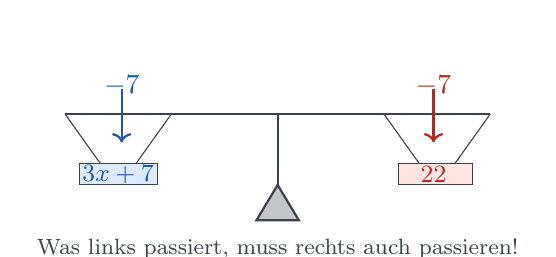
\begin{tikzpicture}[scale=0.9]
  \draw[thick, darkgray] (0,1.5) -- (6,1.5);
  \draw[thick, darkgray] (3,0) -- (3,1.5);
  \draw[thick, darkgray, fill=darkgray!30] (2.7,0) -- (3.3,0) -- (3,0.5) -- cycle;
  \draw[darkgray] (0,1.5) -- (0.5,0.8);
  \draw[darkgray] (1.5,1.5) -- (1.0,0.8);
  \draw[darkgray, fill=lightblue] (0.2,0.5) rectangle (1.3,0.8);
  \node[font=\small\bfseries, mainblue] at (0.75,0.65) {$3x+7$};
  \draw[darkgray] (4.5,1.5) -- (5.0,0.8);
  \draw[darkgray] (6.0,1.5) -- (5.5,0.8);
  \draw[darkgray, fill=lightred] (4.7,0.5) rectangle (5.75,0.8);
  \node[font=\small\bfseries, mainred] at (5.2,0.65) {$22$};
  \node[font=\normalsize, mainblue] at (0.8,1.9) {\textbf{$-7$}};
  \node[font=\normalsize, mainred] at (5.2,1.9) {\textbf{$-7$}};
  \draw[->, mainblue, thick] (0.8,1.85) -- (0.8,1.1);
  \draw[->, mainred, thick] (5.2,1.85) -- (5.2,1.1);
  \node[font=\footnotesize, darkgray, align=center] at (3,-0.4)
    {Was links passiert, muss rechts auch passieren!};
\end{tikzpicture}
\end{center}
\end{visualbox}

\subsection{Terme vereinfachen}

\begin{formulabox}
\[
  \boxed{ax + bx = (a+b)x} \qquad \boxed{a(x+y) = ax + ay}
\]
Gleichartige Terme haben \textbf{dieselbe Variable mit demselben Exponenten}.\\
\textbf{Merke:} $3x$ und $5x$ sind gleichartig $3x$ und $5x^2$ sind \textbf{nicht}!
\end{formulabox}

\begin{examplebox}{Terme zusammenfassen}
\[
  3x + 5y - x + 2y
  = \underbrace{3x - x}_{2x} + \underbrace{5y + 2y}_{7y}
  = 2x + 7y
\]
\[
  4a^2 + 3a - 2a^2 + a = \underbrace{4a^2 - 2a^2}_{2a^2} + \underbrace{3a + a}_{4a} = 2a^2 + 4a
\]
\end{examplebox}

\newpage

\subsection{Klammern aufl\"osen (Distributivgesetz)}

\begin{formulabox}
\[
  \boxed{a \cdot (b + c) = ab + ac} \qquad \boxed{a \cdot (b - c) = ab - ac}
\]
\textbf{Achtung bei negativem Vorzeichen:} $-(x+3) = -x - 3$ \quad (Vorzeichen wechselt!)
\end{formulabox}

\begin{examplebox}{Klammern aufl\"osen -- Schritt f\"ur Schritt}
\begin{align*}
  3(2x - 5) + 4(x + 2) &= 6x - 15 + 4x + 8 \\
                        &= \underbrace{6x + 4x}_{10x} + \underbrace{-15 + 8}_{-7} \\
                        &= 10x - 7
\end{align*}

\vspace{0.3cm}
\textbf{Vorsicht Minusklammer:}
\[
  5x - (3x - 4) = 5x - 3x + 4 = 2x + 4
\]
Das Minus dreht \textbf{alle} Vorzeichen in der Klammer um!
\end{examplebox}

\begin{fehlerbox}
\begin{itemize}
  \item $3(x + 2) \neq 3x + 2$ \quad Richtig: $3(x+2) = 3x + 6$
  \item $-(x - 5) \neq -x - 5$ \quad Richtig: $-(x-5) = -x + 5$
\end{itemize}
\end{fehlerbox}

\subsection{Lineare Gleichungen l\"osen}

\begin{merkbox}
  \textbf{\"Aquivalenzumformungen:} Was man auf einer Seite tut,
  muss man auch auf der anderen tun. Erlaubt: $+$, $-$, $\cdot$, $\div$ (nicht durch 0).
\end{merkbox}

\begin{formulabox}
\[
  \boxed{ax + b = c \quad\Longrightarrow\quad x = \frac{c-b}{a}} \qquad (a \neq 0)
\]
\end{formulabox}

\begin{examplebox}{Lineare Gleichung -- Schritt f\"ur Schritt}
\begin{align*}
  3x + 7 &= 22  &\quad &| -7  \\
  3x     &= 15  &\quad &| \div 3 \\
  x      &= 5
\end{align*}
\textbf{Probe:} $3 \cdot 5 + 7 = 15 + 7 = 22$ \checkmark

\vspace{0.3cm}
\textbf{L\"osung auf dem Zahlenstrahl:}

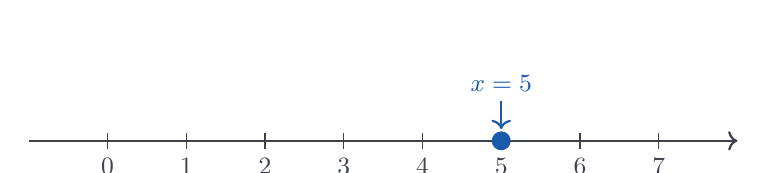
\begin{tikzpicture}
  \draw[->, thick, darkgray] (-1,0) -- (8,0);
  \foreach \i in {0,1,...,7} \draw[darkgray] (\i, 0.1) -- (\i,-0.1) node[below, font=\small] {\i};
  \fill[mainblue] (5,0) circle (0.12);
  \draw[->, mainblue, thick] (5,0.5) -- (5,0.15);
  \node[above, mainblue, font=\small\bfseries] at (5,0.5) {$x = 5$};
\end{tikzpicture}
\end{examplebox}

\begin{examplebox}{Variable auf beiden Seiten}
\begin{align*}
  5x - 3 &= 2x + 9  &\quad &| -2x \\
  3x - 3 &= 9        &\quad &| +3  \\
  3x     &= 12       &\quad &| \div 3 \\
  x      &= 4
\end{align*}
\textbf{Probe:} $5\cdot4 - 3 = 17$ und $2\cdot4 + 9 = 17$ \checkmark
\end{examplebox}

\begin{examplebox}{Gleichung mit Klammern}
\begin{align*}
  2(3x - 1) &= 4x + 8  \\
  6x - 2    &= 4x + 8  & \quad &| -4x \\
  2x - 2    &= 8        & \quad &| +2  \\
  2x        &= 10       & \quad &| \div 2 \\
  x         &= 5
\end{align*}
\textbf{Probe:} $2(3\cdot5-1) = 2\cdot14 = 28$ und $4\cdot5+8 = 28$ \checkmark
\end{examplebox}

\begin{examplebox}{Gleichung mit Bruch}
\[
  \frac{x}{3} + 2 = 5 \qquad | -2
\]
\[
  \frac{x}{3} = 3 \qquad | \cdot 3
\]
\[
  x = 9
\]
\textbf{Tipp:} Bei Bruchgleichungen zuerst den Bruch isolieren, dann mit dem Nenner multiplizieren!
\end{examplebox}

\subsection{Gleichungssysteme (zwei Gleichungen)}

\begin{merkbox}
Zwei Gleichungen, zwei Unbekannte -- wir suchen einen \textbf{Punkt}, der auf
\textit{beiden} Geraden liegt (Schnittpunkt). Es gibt drei L\"osungsverfahren:
\begin{itemize}
  \item \textbf{Gleichsetzungsverfahren:} Beide nach $y$ aufl\"osen, gleichsetzen
  \item \textbf{Additionsverfahren:} Eine Variable ausdr\"ucken, einsetzen
  \item \textbf{Einsetzungsverfahren:} Gleichungen addieren, eine Variable eliminieren
\end{itemize}
\end{merkbox}

\begin{examplebox}{Gleichsetzungsverfahren -- mit Grafik}
\begin{align*}
  \text{I:}  &\quad y = 2x + 1 \\
  \text{II:} &\quad y = -x + 7
\end{align*}
Gleichsetzen: $2x+1 = -x+7 \;\Rightarrow\; 3x=6 \;\Rightarrow\; x=2$\\
Einsetzen: $y = 2\cdot2+1 = 5$ \quad $\Rightarrow$ \textbf{L\"osung: } $L(2\mid 5)$

\vspace{0.4cm}
\begin{center}
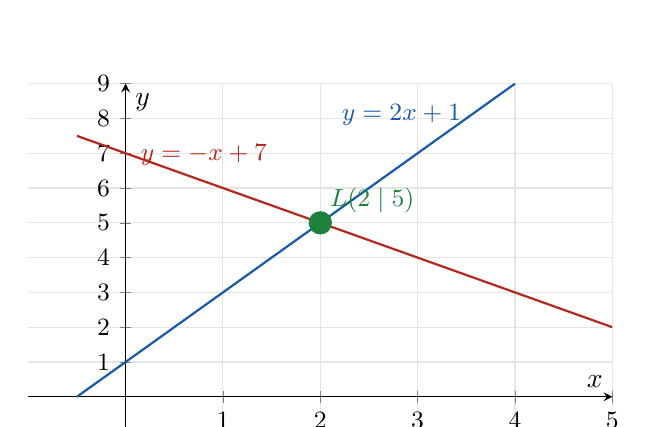
\begin{tikzpicture}
  \begin{axis}[
    width=9cm, height=6cm,
    xmin=-1, xmax=5, ymin=-1, ymax=9,
    axis lines=middle,
    xlabel={$x$}, ylabel={$y$},
    grid=major, grid style={gray!20},
    tick label style={font=\small},
    xtick={0,1,...,5}, ytick={0,1,...,9},
  ]
    \addplot[mainblue, thick, domain=-0.5:4] {2*x+1}
      node[left, pos=0.9, font=\small] {$y=2x+1$};
    \addplot[mainred, thick, domain=-0.5:5] {-x+7}
      node[right, pos=0.1, font=\small] {$y=-x+7$};
    \addplot[maingreen, mark=*, mark size=4pt, only marks]
      coordinates {(2,5)};
    \node[maingreen, font=\small\bfseries,above right] at (axis cs:2,5)
      {$L(2\mid 5)$};
  \end{axis}
\end{tikzpicture}
\end{center}
\end{examplebox}

\begin{examplebox}{Additionsverfahren}
\begin{align*}
  \text{I:}  &\quad 2x + 3y = 12 \\
  \text{II:} &\quad 4x - 3y = 6
\end{align*}
I $+$ II: \quad $6x = 18 \;\Rightarrow\; x = 3$\\
In I einsetzen: $2\cdot3 + 3y = 12 \;\Rightarrow\; 3y = 6 \;\Rightarrow\; y = 2$\\
\textbf{L\"osung:} $L(3\mid 2)$ \quad \textbf{Probe I:} $6+6=12$ \checkmark \quad \textbf{Probe II:} $12-6=6$ \checkmark
\end{examplebox}

\begin{examplebox}{Einsetzungsverfahren}
	\begin{align*}
		\text{I:}  &\quad y = 3x - 1 \\
		\text{II:} &\quad 2x + y = 9
	\end{align*}
	\textbf{Schritt 1:} Gleichung I gibt uns $y$ bereits fertig: $y = 3x - 1$\\[0.2cm]
	\textbf{Schritt 2:} $y$ in Gleichung II \textbf{einsetzen}:
	\[
	2x + (3x - 1) = 9
	\]
	\textbf{Schritt 3:} Aufl\"osen nach $x$:
	\begin{align*}
		5x - 1 &= 9  &\quad &| +1 \\
		5x     &= 10 &\quad &| \div 5 \\
		x      &= 2
	\end{align*}
	\textbf{Schritt 4:} $x = 2$ in Gleichung I einsetzen:
	\[
	y = 3 \cdot 2 - 1 = \mathbf{5}
	\]
	\textbf{L\"osung:} $L(2 \mid 5)$\\
	\textbf{Probe I:} $5 = 3\cdot2-1 = 5$ \checkmark \quad
	\textbf{Probe II:} $2\cdot2+5 = 9$ \checkmark
\end{examplebox}

\newpage

\subsection{\"Ubungsaufgaben -- Gleichungen}

\exercise{L\"osung gesucht: $4x - 5 = 19$\\[0.8cm]
  \textit{L\"osung:} \dotfill}

\exercise{L\"osung gesucht: $2(x + 3) = 3x - 1$\\[0.8cm]
  \textit{L\"osung:} \dotfill}

\exercise{L\"osung gesucht: $\dfrac{x}{3} + 4 = 7$\\[0.8cm]
  \textit{L\"osung:} \dotfill}

\exercise{Variable auf beiden Seiten: $6x + 2 = 2x + 18$\\[0.8cm]
  \textit{L\"osung:} \dotfill}

\exercise{Klammern aufl\"osen und l\"osen: $3(2x-1) - 2(x+4) = 5$\\[0.8cm]
  \textit{L\"osung:} \dotfill}

\exercise{Gleichungssystem l\"osen: I: $y = 3x - 2$ \quad II: $y = -2x + 8$\\[1.0cm]
  \textit{L\"osung:} \dotfill}

\exercise{Additionsverfahren: I: $3x + 2y = 11$ \quad II: $x - 2y = 1$\\[1.0cm]
  \textit{L\"osung:} \dotfill}

\newpage
% ============================================================
\section{\color{mainblue}Funktionen}
% ============================================================

\subsection{Was ist eine Funktion?}

Eine \textbf{Funktion} ordnet jedem $x$-Wert \textbf{genau einen} $y$-Wert zu.
Man schreibt $y = \ldots$ oder $f(x) = \ldots$

\begin{visualbox}
\textbf{Funktion als Maschine:}

\begin{center}
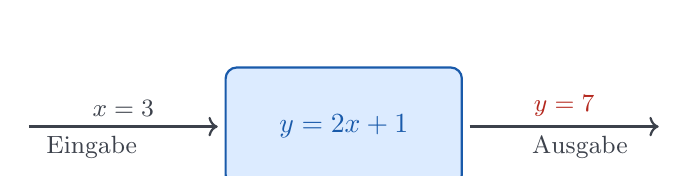
\begin{tikzpicture}
  \draw[mainblue, thick, fill=lightblue, rounded corners=4pt]
    (2.5,0) rectangle (5.5,1.5);
  \node[mainblue, font=\bfseries] at (4,0.75) {$y = 2x + 1$};
  \draw[->, thick, darkgray] (0,0.75) -- (2.4,0.75);
  \node[above, font=\small\bfseries, darkgray] at (1.2,0.75) {$x = 3$};
  \draw[->, thick, darkgray] (5.6,0.75) -- (8,0.75);
  \node[above, font=\small\bfseries, mainred] at (6.8,0.75) {$y = 7$};
  \node[below, font=\small, darkgray] at (0.8,0.75) {Eingabe};
  \node[below, font=\small, darkgray] at (7.0,0.75) {Ausgabe};
\end{tikzpicture}
\end{center}
\end{visualbox}

\begin{tipbox}
\textbf{Funktionswert berechnen:} Einfach $x$ durch die Zahl ersetzen!\\
Beispiel: $f(x) = 3x - 2$\\
$f(4) = 3\cdot4 - 2 = 12 - 2 = \mathbf{10}$\\
$f(0) = 3\cdot0 - 2 = \mathbf{-2}$ \quad (das ist der y-Achsenabschnitt!)\\
$f(-1) = 3\cdot(-1) - 2 = -3 - 2 = \mathbf{-5}$
\end{tipbox}

\subsection{Lineare Funktionen}

Eine \textbf{lineare Funktion} beschreibt eine Gerade im Koordinatensystem.

\begin{formulabox}
\[
  \boxed{y = mx + b}
\]
\begin{itemize}
  \item $m$ = \textbf{Steigung} -- wie steil ist die Gerade?
  \item $b$ = \textbf{y-Achsenabschnitt} -- wo schneidet sie die y-Achse (bei $x=0$)?
\end{itemize}
\end{formulabox}

\begin{visualbox}
\textbf{Das Steigungsdreieck -- so liest man $m$ aus dem Graphen ab:}

\begin{center}
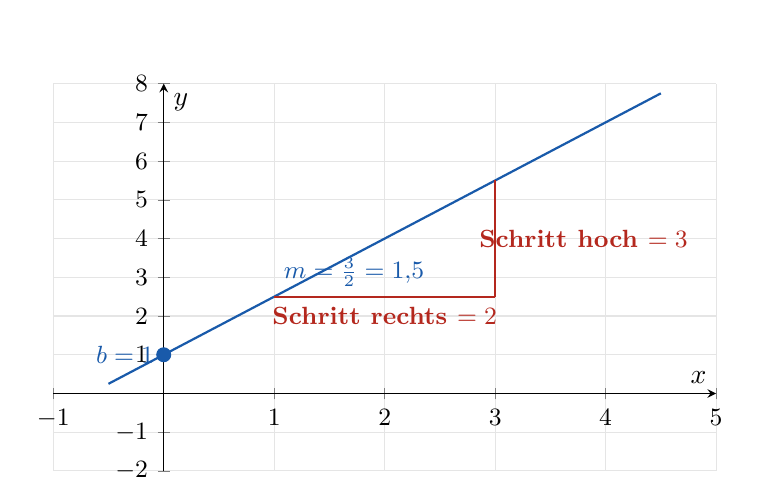
\begin{tikzpicture}
  \begin{axis}[
    width=10cm, height=6.5cm,
    xmin=-1, xmax=5, ymin=-2, ymax=8,
    axis lines=middle,
    xlabel={$x$}, ylabel={$y$},
    xtick={-1,0,...,5}, ytick={-2,-1,...,8},
    grid=major, grid style={gray!20},
    tick label style={font=\small},
  ]
    \addplot[mainblue, thick, domain=-0.5:4.5] {1.5*x + 1};
    \addplot[mainred, thick] coordinates {(1,2.5)(3,2.5)};
    \addplot[mainred, thick] coordinates {(3,2.5)(3,5.5)};
    \node[mainred, font=\small\bfseries] at (axis cs:2,2.0) {Schritt rechts $= 2$};
    \node[mainred, font=\small\bfseries] at (axis cs:3.8,4.0) {Schritt hoch $= 3$};
    \node[mainblue, font=\small, above right] at (axis cs:1,2.5)
      {$m = \frac{3}{2} = 1{,}5$};
    \addplot[mainblue, fill=mainblue, mark=*, mark size=2.5pt]
      coordinates {(0,1)};
    \node[mainblue, font=\small\bfseries, left] at (axis cs:0,1) {$b=1$};
  \end{axis}
\end{tikzpicture}
\end{center}
\end{visualbox}

\begin{center}
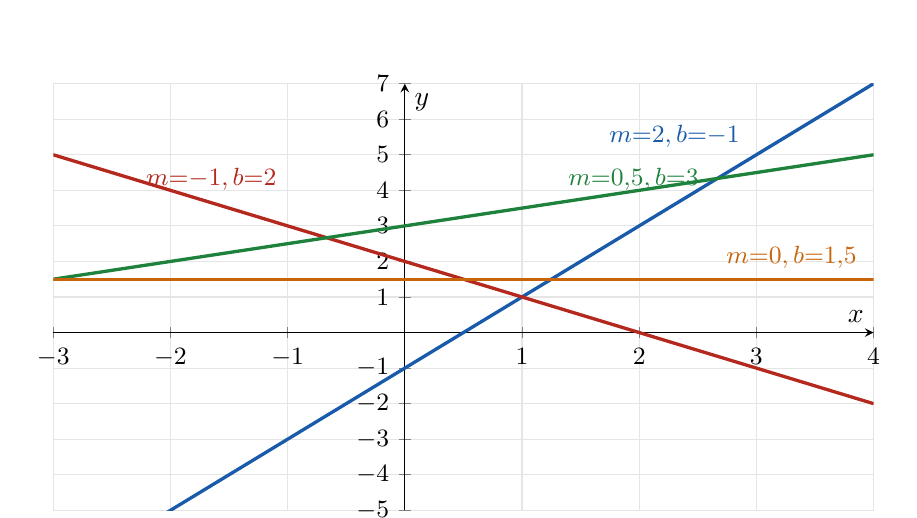
\begin{tikzpicture}
  \begin{axis}[
    width=12cm, height=7cm,
    xmin=-3, xmax=4, ymin=-5, ymax=7,
    axis lines=middle,
    xlabel={$x$}, ylabel={$y$},
    xtick={-3,-2,...,4}, ytick={-5,-4,...,7},
    grid=major, grid style={gray!20},
    tick label style={font=\small},
    legend pos=north west,
    legend style={font=\small},
  ]
    \addplot[mainblue, very thick, domain=-3:4] {2*x - 1}
      node[above left, pos=0.85, font=\small] {$m{=}2, b{=}{-1}$};
    \addplot[mainred, very thick, domain=-3:4] {-x + 2}
      node[right, pos=0.1, font=\small] {$m{=}{-1}, b{=}2$};
    \addplot[maingreen, very thick, domain=-3:4] {0.5*x + 3}
      node[left, pos=0.8, font=\small] {$m{=}0{,}5, b{=}3$};
    \addplot[mainorange, very thick, domain=-3:4] {1.5}
      node[above, pos=0.9, font=\small] {$m{=}0, b{=}1{,}5$};
  \end{axis}
\end{tikzpicture}
\end{center}

\begin{merkbox}
\begin{itemize}
  \item $m > 0$: Gerade \textbf{steigt} \quad $m < 0$: Gerade \textbf{f\"allt} \quad $m = 0$: \textbf{waagerecht}
  \item \textbf{Gr\"osseres $|m|$} = steilere Gerade
  \item \textbf{$b > 0$}: y-Achse wird oben geschnitten \quad \textbf{$b < 0$}: unten geschnitten
  \item \textbf{Parallele Geraden} haben \textbf{denselben} $m$-Wert, aber verschiedenes $b$
\end{itemize}
\end{merkbox}

\begin{formulabox}
\textbf{Steigung aus zwei Punkten:}
\[
  \boxed{m = \frac{y_2 - y_1}{x_2 - x_1}}
\]
\textbf{Nullstelle} (wo schneidet die Gerade die x-Achse?): $y = 0$ setzen und $x$ berechnen.\\
\textbf{y-Achsenabschnitt:} $x = 0$ setzen $\;\Rightarrow\; y = b$
\end{formulabox}

\begin{examplebox}{Geradengleichung aus zwei Punkten}
Gegeben: $P_1(1\mid 3)$ und $P_2(4\mid 9)$
\[
  m = \frac{9-3}{4-1} = \frac{6}{3} = 2
\]
Einsetzen in $y = mx + b$ mit $P_1$: \quad $3 = 2\cdot1 + b \;\Rightarrow\; b = 1$\\[0.2cm]
\textbf{Ergebnis:} $\boxed{y = 2x + 1}$
\end{examplebox}

\begin{examplebox}{Nullstelle und Achsenabschnitt berechnen}
Gegeben: $y = 3x - 6$

\textbf{Nullstelle} (y = 0):
\[
  0 = 3x - 6 \;\Rightarrow\; 3x = 6 \;\Rightarrow\; x = 2 \quad \Rightarrow \text{Nullstelle bei } N(2\mid0)
\]
\textbf{y-Achsenabschnitt} (x = 0):
\[
  y = 3\cdot0 - 6 = -6 \quad \Rightarrow \text{y-Achsenabschnitt: } (0\mid -6)
\]
\end{examplebox}

\newpage

\subsection{\"Ubungsaufgaben -- Funktionen}

\exercise{Bestimme Steigung und y-Achsenabschnitt durch $P_1(0\mid 2)$ und $P_2(3\mid 8)$.\\[0.8cm]
  \textit{L\"osung:} \dotfill}

\exercise{Zeichne $y = -2x + 5$ in ein Koordinatensystem. Wo schneidet die Gerade die Achsen?\\[3.0cm]}

\exercise{Berechne $f(3)$, $f(-2)$ und $f(0)$ f\"ur $f(x) = 4x - 3$.\\[0.8cm]
  \textit{L\"osung:} \dotfill}

\exercise{Erstelle eine Wertetabelle f\"ur $y = 5x - 3$ mit $x \in \{-2,-1,0,1,2\}$ und zeichne die Parabel.\\[3.5cm]}

\exercise{Welche Geradengleichung hat dieselbe Steigung wie $y = 3x + 1$, aber schneidet die y-Achse bei $-4$?\\[0.8cm]
  \textit{L\"osung:} \dotfill}

\newpage
% ============================================================
\section{\color{mainblue}Winkel}
% ============================================================

\subsection{Was ist ein Winkel?}

Ein \textbf{Winkel} entsteht, wenn zwei Strahlen oder Geraden vom selben Punkt ausgehen.
Der Schnittpunkt heisst \textbf{Scheitel}. Winkel werden in \textbf{Grad} ($^\circ$) gemessen.

\begin{visualbox}
\textbf{Aufbau eines Winkels:}

\begin{center}
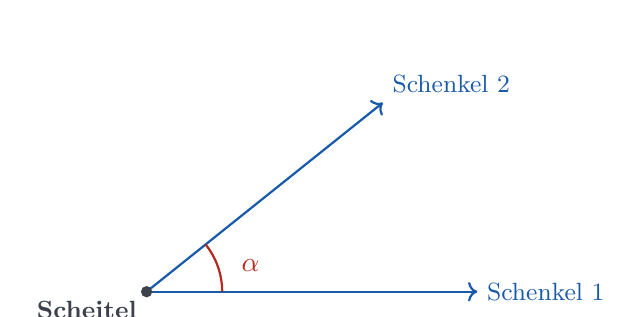
\begin{tikzpicture}[scale=1.2]
  % Two rays
  \draw[->, thick, mainblue] (0,0) -- (3.5,0);
  \draw[->, thick, mainblue] (0,0) -- (2.5,2.0);
  % Angle arc
  \draw[mainred, thick] (0.8,0) arc[start angle=0, end angle=38.66, radius=0.8];
  % Label
  \node[mainred, font=\bfseries] at (1.1,0.28) {$\alpha$};
  % Vertex label
  \node[below left, darkgray, font=\small\bfseries] at (0,0) {Scheitel};
  \fill[darkgray] (0,0) circle (0.06);
  % Rays labels
  \node[right, mainblue, font=\small] at (3.5,0) {Schenkel 1};
  \node[above right, mainblue, font=\small] at (2.5,2.0) {Schenkel 2};
\end{tikzpicture}
\end{center}
\end{visualbox}

\subsection{Die Winkelarten -- \"Uberblick}

\begin{merkbox}
Es gibt \textbf{sechs} Grundtypen von Winkeln -- du musst alle kennen und benennen k\"onnen!
\end{merkbox}

\subsubsection*{1. Spitzwinkel}

\begin{winkelbox}
\textbf{Spitzwinkel:} $0^\circ < \alpha < 90^\circ$ \quad (kleiner als ein rechter Winkel)
\end{winkelbox}

\begin{center}
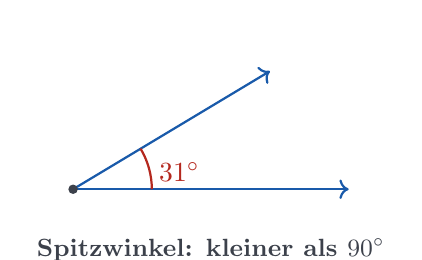
\begin{tikzpicture}
  \draw[->, thick, mainblue] (0,0) -- (3.5,0);
  \draw[->, thick, mainblue] (0,0) -- (2.5,1.5);
  \draw[mainred, thick] (1.0,0) arc[start angle=0, end angle=31, radius=1.0];
  \node[mainred, font=\bfseries] at (1.35,0.22) {$31^\circ$};
  \fill[darkgray] (0,0) circle (0.06);
  \node[below, darkgray, font=\small\bfseries] at (1.75,-0.5) {Spitzwinkel: kleiner als $90^\circ$};
\end{tikzpicture}
\end{center}

\subsubsection*{2. Rechter Winkel}

\begin{winkelbox}
\textbf{Rechter Winkel:} $\alpha = 90^\circ$ \quad (wird mit dem Quadrat $\square$ markiert!)
\end{winkelbox}

\begin{center}
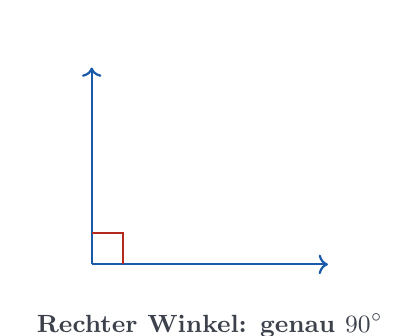
\begin{tikzpicture}
  \draw[->, thick, mainblue] (0,0) -- (3.0,0);
  \draw[->, thick, mainblue] (0,0) -- (0,2.5);
  \draw[mainred, thick] (0.4,0) -- (0.4,0.4) -- (0,0.4);
  \node[below, darkgray, font=\small\bfseries] at (1.5,-0.5) {Rechter Winkel: genau $90^\circ$};
\end{tikzpicture}
\end{center}

\subsubsection*{3. Stumpfer Winkel}

\begin{winkelbox}
\textbf{Stumpfer Winkel:} $90^\circ < \alpha < 180^\circ$ \quad (gr\"osser als rechter, kleiner als gestreckt)
\end{winkelbox}

\begin{center}
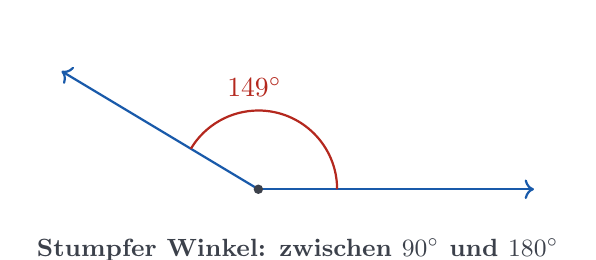
\begin{tikzpicture}
  \draw[->, thick, mainblue] (0,0) -- (3.5,0);
  \draw[->, thick, mainblue] (0,0) -- (-2.5,1.5);
  \draw[mainred, thick] (1.0,0) arc[start angle=0, end angle=149, radius=1.0];
  \node[mainred, font=\bfseries] at (-0.05,1.3) {$149^\circ$};
  \fill[darkgray] (0,0) circle (0.06);
  \node[below, darkgray, font=\small\bfseries] at (0.5,-0.5) {Stumpfer Winkel: zwischen $90^\circ$ und $180^\circ$};
\end{tikzpicture}
\end{center}

\subsubsection*{4. Gestreckter Winkel (Flachwinkel)}

\begin{winkelbox}
\textbf{Gestreckter Winkel / Flachwinkel:} $\alpha = 180^\circ$ \quad (eine gerade Linie!)
\end{winkelbox}

\begin{center}
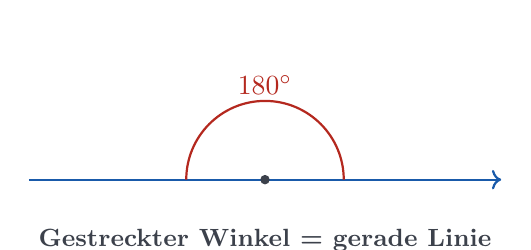
\begin{tikzpicture}
  \draw[->, thick, mainblue] (-3.0,0) -- (3.0,0);
  \draw[mainred, thick] (1.0,0) arc[start angle=0, end angle=180, radius=1.0];
  \node[mainred, font=\bfseries] at (0,1.2) {$180^\circ$};
  \fill[darkgray] (0,0) circle (0.06);
  \node[below, darkgray, font=\small\bfseries] at (0,-0.5) {Gestreckter Winkel = gerade Linie};
\end{tikzpicture}
\end{center}

\subsubsection*{5. \"Uberstumpfer Winkel}

\begin{winkelbox}
\textbf{\"Uberstumpfer Winkel:} $180^\circ < \alpha < 360^\circ$ \quad (auch: Reflexwinkel)
\end{winkelbox}

\begin{center}
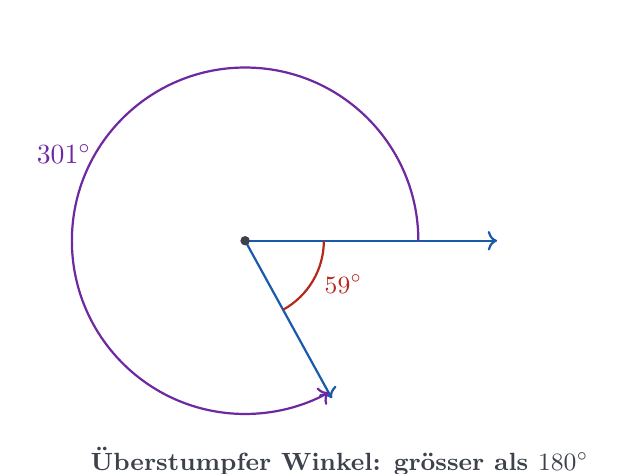
\begin{tikzpicture}
  % Two rays from origin
  \draw[->, thick, mainblue] (0,0) -- (3.2,0);
  \draw[->, thick, mainblue] (0,0) -- (1.1,-2.0);
  \fill[darkgray] (0,0) circle (0.06);
  % Small inner angle (acute, below x-axis)
  \draw[mainred, thick] (1.0,0) arc[start angle=0, end angle=-61, radius=1.0];
  \node[mainred, font=\small] at (1.25,-0.55) {$59^\circ$};
  % Reflex angle label with a curved arrow going the long way (above)
  \draw[mainpurple, thick, ->]
    (2.2,0) arc[start angle=0, end angle=299, radius=2.2];
  \node[mainpurple, font=\bfseries] at (-2.3, 1.1) {$301^\circ$};
  \node[below, darkgray, font=\small\bfseries] at (1.2,-2.5)
    {\"Uberstumpfer Winkel: gr\"osser als $180^\circ$};
\end{tikzpicture}
\end{center}

\subsubsection*{6. Vollwinkel}

\begin{winkelbox}
\textbf{Vollwinkel:} $\alpha = 360^\circ$ \quad (eine volle Umdrehung)
\end{winkelbox}

\begin{center}
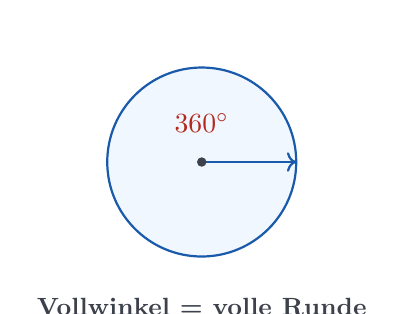
\begin{tikzpicture}
  \draw[mainblue, thick, fill=lightblue!40] (0,0) circle (1.2cm);
  \draw[->, thick, mainblue] (0,0) -- (1.2,0);
  \fill[darkgray] (0,0) circle (0.06);
  \node[mainred, font=\bfseries] at (0,0.5) {$360^\circ$};
  \node[below, darkgray, font=\small\bfseries] at (0,-1.6) {Vollwinkel = volle Runde};
\end{tikzpicture}
\end{center}

\vspace{0.4cm}

\begin{center}
\renewcommand{\arraystretch}{1.6}
\begin{tabular}{>{\bfseries}p{4.2cm} p{3.5cm} p{5cm}}
  \toprule
  \textbf{Winkelart} & \textbf{Gr\"osse} & \textbf{Erkennungsmerkmal} \\
  \midrule
  Spitzwinkel        & $0^\circ < \alpha < 90^\circ$   & ``spitz'', kleiner als rechter Winkel \\
  Rechter Winkel     & $\alpha = 90^\circ$              & Quadrat-Symbol $\square$ \\
  Stumpfer Winkel    & $90^\circ < \alpha < 180^\circ$  & breiter als rechter Winkel \\
  Gestreckter Winkel & $\alpha = 180^\circ$             & gerade Linie \\
  \"Uberstumpfer Winkel & $180^\circ < \alpha < 360^\circ$ & ``mehr als halb rum'' \\
  Vollwinkel         & $\alpha = 360^\circ$             & volle Runde \\
  \bottomrule
\end{tabular}
\end{center}

\subsection{Winkelpaare -- Zwei Winkel, eine Beziehung}

\subsubsection*{Scheitelwinkel}

\begin{winkelbox}
Wenn sich zwei Geraden schneiden, entstehen \textbf{vier Winkel}.
Winkel, die \textbf{gegen\"uber} liegen, heissen \textbf{Scheitelwinkel} -- sie sind \textbf{gleich gross}!
\[
  \boxed{\alpha = \gamma \qquad \beta = \delta}
\]
\end{winkelbox}

\begin{center}
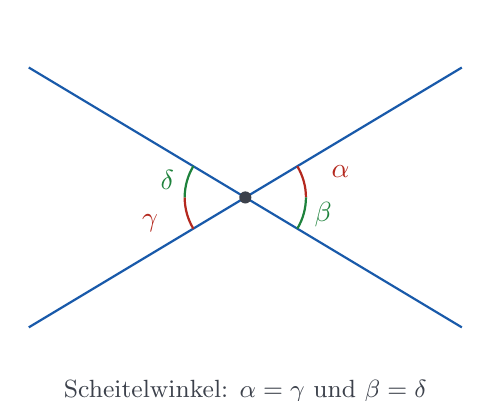
\begin{tikzpicture}[scale=1.1]
  \draw[thick, mainblue] (-2.5,-1.5) -- (2.5,1.5);
  \draw[thick, mainblue] (-2.5,1.5) -- (2.5,-1.5);
  \fill[darkgray] (0,0) circle (0.07);
  % Arcs for angles
  \draw[mainred, thick] (0.7,0) arc[start angle=0, end angle=31, radius=0.7];
  \draw[mainred, thick] (-0.7,0) arc[start angle=180, end angle=211, radius=0.7];
  \draw[maingreen, thick] (0.7,0) arc[start angle=0, end angle=-31, radius=0.7];
  \draw[maingreen, thick] (-0.7,0) arc[start angle=180, end angle=149, radius=0.7];
  % Labels
  \node[mainred, font=\bfseries] at (1.1,0.3) {$\alpha$};
  \node[mainred, font=\bfseries] at (-1.1,-0.3) {$\gamma$};
  \node[maingreen, font=\bfseries] at (0.9,-0.2) {$\beta$};
  \node[maingreen, font=\bfseries] at (-0.9,0.2) {$\delta$};
  \node[below, darkgray, font=\small] at (0,-2.0)
    {Scheitelwinkel: $\alpha = \gamma$ und $\beta = \delta$};
\end{tikzpicture}
\end{center}

\subsubsection*{Nebenwinkel}

\begin{winkelbox}
\textbf{Nebenwinkel} liegen \textbf{nebeneinander} auf einer geraden Linie.\\
Ihre Summe betr\"agt immer $\mathbf{180^\circ}$!
\[
  \boxed{\alpha + \beta = 180^\circ}
\]
\end{winkelbox}

\begin{center}
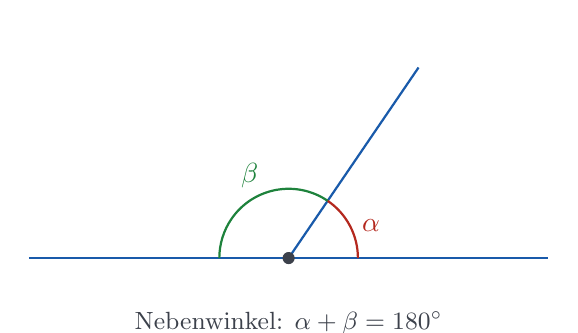
\begin{tikzpicture}[scale=1.1]
  \draw[thick, mainblue] (-3,0) -- (3,0);
  \draw[thick, mainblue] (0,0) -- (1.5,2.2);
  \fill[darkgray] (0,0) circle (0.07);
  % alpha: from 0° to ~55.7°
  \draw[mainred, thick] (0.8,0) arc[start angle=0, end angle=55.7, radius=0.8];
  % beta: from 55.7° to 180° (single arc, no overlap)
  \draw[maingreen, thick] ({0.8*cos(55.7)},{0.8*sin(55.7)})
    arc[start angle=55.7, end angle=180, radius=0.8];
  \node[mainred, font=\bfseries] at (0.95, 0.38) {$\alpha$};
  \node[maingreen, font=\bfseries] at (-0.45, 0.95) {$\beta$};
  \node[below, darkgray, font=\small] at (0,-0.5)
    {Nebenwinkel: $\alpha + \beta = 180^\circ$};
\end{tikzpicture}
\end{center}

\begin{examplebox}{Nebenwinkel berechnen}
Ein Nebenwinkel betr\"agt $\alpha = 65^\circ$. Wie gross ist $\beta$?
\[
  \beta = 180^\circ - \alpha = 180^\circ - 65^\circ = \mathbf{115^\circ}
\]
\end{examplebox}

\subsubsection*{Komplementwinkel und Supplementwinkel}

\begin{formulabox}
\[
  \textbf{Komplementwinkel:} \quad \alpha + \beta = 90^\circ \quad \Rightarrow \quad \beta = 90^\circ - \alpha
\]
\[
  \textbf{Supplementwinkel:} \quad \alpha + \beta = 180^\circ \quad \Rightarrow \quad \beta = 180^\circ - \alpha
\]
\textbf{Eselsbrücke:} \textbf{K}omplementär = \textbf{K}urz (90°) \quad \textbf{S}upplementär = \textbf{S}treck (180°)
\end{formulabox}

\begin{examplebox}{Komplementwinkel und Supplementwinkel}
Gegeben: $\alpha = 40^\circ$\\[0.2cm]
\textbf{Komplementwinkel:} $\beta = 90^\circ - 40^\circ = 50^\circ$\\
\textbf{Supplementwinkel:} $\gamma = 180^\circ - 40^\circ = 140^\circ$
\end{examplebox}

\subsection{Winkel an Parallelen}

Wenn eine \textbf{Quergerade} (Transversale) zwei parallele Geraden schneidet,
entstehen besondere Winkelbeziehungen. Das musst du kennen!

\begin{center}
\begin{tikzpicture}[scale=1.0]
  % Two parallel lines
  \draw[thick, mainblue] (-2.5, 1.5) -- (4.0, 1.5) node[right, font=\small] {$g_1$};
  \draw[thick, mainblue] (-2.5,-1.5) -- (4.0,-1.5) node[right, font=\small] {$g_2$};
  % Transversal: from (-0.5,-3) to (2.5,3), slope=2
  % Intersections: y=1.5 -> x=1.75;  y=-1.5 -> x=0.25
  \draw[thick, mainred] (-0.5,-3) -- (2.5,3);
  % Intersection dots at correct positions
  \fill[darkgray] (1.75, 1.5) circle (0.07);
  \fill[darkgray] (0.25,-1.5) circle (0.07);
  % Angle = arctan(2) ≈ 63.4°
  % Angles at upper intersection (1.75, 1.5)
  \draw[mainred, thick]    (1.75,1.5) ++(0.55,0) arc[start angle=0,   end angle=63.4,  radius=0.55];
  \draw[mainred, thick]    (1.75,1.5) ++(-0.55,0) arc[start angle=180, end angle=243.4, radius=0.55];
  \draw[maingreen, thick]  (1.75,1.5) ++(0.45,0) arc[start angle=0,   end angle=-116.6, radius=0.45];
  \draw[maingreen, thick]  (1.75,1.5) ++(-0.45,0) arc[start angle=180, end angle=63.4,  radius=0.45];
  \node[mainred,   font=\bfseries] at (2.55, 1.85) {$\alpha$};
  \node[mainred,   font=\bfseries] at (0.90, 1.15) {$\gamma$};
  \node[maingreen, font=\bfseries] at (2.35, 1.05) {$\beta$};
  \node[maingreen, font=\bfseries] at (1.15, 1.90) {$\delta$};
  % Angles at lower intersection (0.25, -1.5) — dashed to show correspondence
  \draw[mainred, dashed, thick]   (0.25,-1.5) ++(0.55,0) arc[start angle=0,   end angle=63.4,  radius=0.55];
  \draw[mainteal, thick]          (0.25,-1.5) ++(-0.55,0) arc[start angle=180, end angle=63.4, radius=0.55];
  \node[mainred,   font=\bfseries] at (1.05,-1.15) {$\alpha$};
  \node[mainteal,  font=\bfseries] at (-0.55,-1.15) {$\delta$};
\end{tikzpicture}
\end{center}

\subsubsection*{Stufenwinkel (F-Winkel)}

\begin{winkelbox}
\textbf{Stufenwinkel} liegen auf \textbf{derselben Seite} der Quergerade und auf \textbf{verschiedenen} parallelen Geraden -- sie sehen wie ein ``F'' aus.\\[0.2cm]
\[
  \boxed{\text{Stufenwinkel sind gleich gross!} \quad \alpha = \alpha}
\]
\end{winkelbox}

\begin{center}
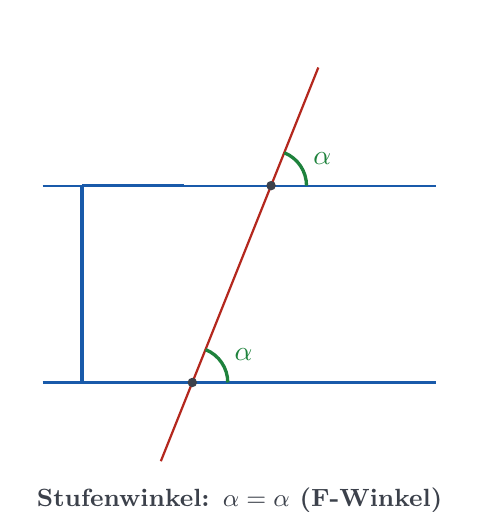
\begin{tikzpicture}[scale=1.0]
  \draw[thick, mainblue] (-1, 1.5) -- (4, 1.5);
  \draw[thick, mainblue] (-1,-1.0) -- (4,-1.0);
  \draw[thick, mainred] (0.5,-2) -- (2.5,3);
  % F-shape highlight
  \draw[mainblue, very thick] (-0.5,1.5) -- (0.8,1.5);
  \draw[mainblue, very thick] (-0.5,-1.0) -- (0.7,-1.0);
  \draw[mainblue, very thick] (-0.5,-1.0) -- (-0.5,1.5);
  % Correct intersections: upper=(1.9,1.5), lower=(0.9,-1.0), angle=68.2°
  \fill[darkgray] (1.9, 1.5) circle (0.06);
  \fill[darkgray] (0.9,-1.0) circle (0.06);
  % Angle arcs (same position, same angle = Stufenwinkel)
  \draw[maingreen, very thick] (1.9,1.5) ++(0.45,0) arc[start angle=0, end angle=68, radius=0.45];
  \draw[maingreen, very thick] (0.9,-1.0) ++(0.45,0) arc[start angle=0, end angle=68, radius=0.45];
  \node[maingreen, font=\bfseries] at (2.55, 1.85) {$\alpha$};
  \node[maingreen, font=\bfseries] at (1.55,-0.65) {$\alpha$};
  \node[darkgray, font=\small\bfseries] at (1.5,-2.5) {Stufenwinkel: $\alpha = \alpha$ (F-Winkel)};
\end{tikzpicture}
\end{center}

\newpage

\subsubsection*{Wechselwinkel (Z-Winkel)}

\begin{winkelbox}
\textbf{Wechselwinkel} liegen auf \textbf{verschiedenen Seiten} der Quergerade und \textbf{zwischen} den Parallelen -- sie sehen wie ein ``Z'' (oder ``N'') aus.\\[0.2cm]
\[
  \boxed{\text{Wechselwinkel sind gleich gross!} \quad \alpha = \beta}
\]
\end{winkelbox}

\begin{center}
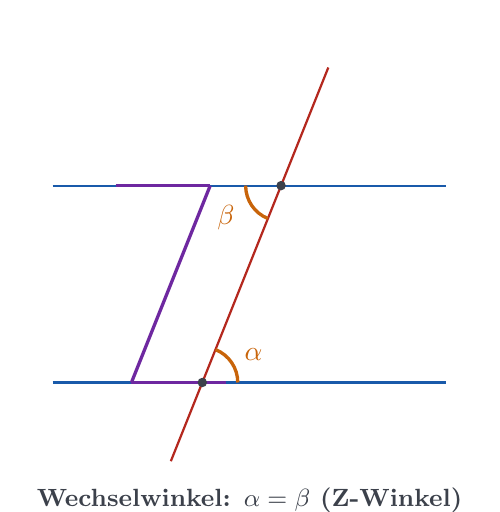
\begin{tikzpicture}[scale=1.0]
  \draw[thick, mainblue] (-1, 1.5) -- (4, 1.5);
  \draw[thick, mainblue] (-1,-1.0) -- (4,-1.0);
  \draw[thick, mainred] (0.5,-2) -- (2.5,3);
  % Z-shape highlight
  \draw[mainpurple, very thick] (-0.2,1.5) -- (1.0,1.5);
  \draw[mainpurple, very thick] (0.0,-1.0) -- (1.2,-1.0);
  \draw[mainpurple, very thick] (1.0,1.5) -- (0.0,-1.0);
  % Correct intersections: upper=(1.9,1.5), lower=(0.9,-1.0), angle=68.2°
  \fill[darkgray] (1.9, 1.5) circle (0.06);
  \fill[darkgray] (0.9,-1.0) circle (0.06);
  % Upper: arc on LEFT side of transversal (180° to 180°+68°=248°)
  \draw[mainorange, very thick] (1.9,1.5) ++(-0.45,0) arc[start angle=180, end angle=248, radius=0.45];
  % Lower: arc on RIGHT side of transversal (0° to 68°)
  \draw[mainorange, very thick] (0.9,-1.0) ++(0.45,0) arc[start angle=0, end angle=68, radius=0.45];
  \node[mainorange, font=\bfseries] at (1.2, 1.1) {$\beta$};
  \node[mainorange, font=\bfseries] at (1.55,-0.65) {$\alpha$};
  \node[darkgray, font=\small\bfseries] at (1.5,-2.5) {Wechselwinkel: $\alpha = \beta$ (Z-Winkel)};
\end{tikzpicture}
\end{center}

\subsubsection*{Gleichsinnige Winkel (Co-interior Winkel)}

\begin{winkelbox}
\textbf{Gleichsinnige Winkel} liegen \textbf{zwischen} den Parallelen auf \textbf{derselben Seite} der Quergerade.\\[0.2cm]
\[
  \boxed{\text{Gleichsinnige Winkel erg\"anzen sich zu } 180^\circ! \quad \alpha + \beta = 180^\circ}
\]
\end{winkelbox}

\begin{center}
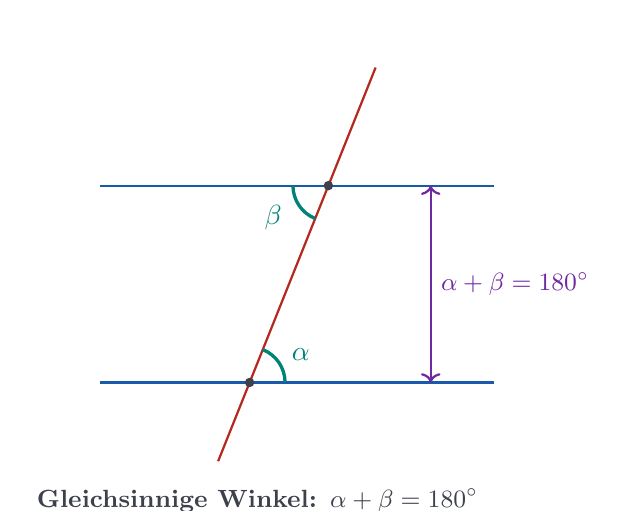
\begin{tikzpicture}[scale=1.0]
  \draw[thick, mainblue] (-1, 1.5) -- (4, 1.5);
  \draw[thick, mainblue] (-1,-1.0) -- (4,-1.0);
  \draw[thick, mainred] (0.5,-2) -- (2.5,3);
  % Correct intersections: upper=(1.9,1.5), lower=(0.9,-1.0), angle=68.2°
  \fill[darkgray] (1.9, 1.5) circle (0.06);
  \fill[darkgray] (0.9,-1.0) circle (0.06);
  % Upper: arc on LEFT of transversal = 180° to 248° (same side as lower right)
  \draw[mainteal, very thick] (1.9,1.5) ++(-0.45,0) arc[start angle=180, end angle=248, radius=0.45];
  % Lower: arc on RIGHT of transversal = 0° to 68°
  \draw[mainteal, very thick] (0.9,-1.0) ++(0.45,0) arc[start angle=0, end angle=68, radius=0.45];
  \node[mainteal, font=\bfseries] at (1.2, 1.1) {$\beta$};
  \node[mainteal, font=\bfseries] at (1.55,-0.65) {$\alpha$};
  % Annotation showing they add to 180°
  \draw[mainpurple, <->, thick] (3.2,1.5) -- (3.2,-1.0)
    node[midway, right, font=\small, mainpurple] {$\alpha+\beta=180^\circ$};
  \node[darkgray, font=\small\bfseries] at (1.0,-2.5) {Gleichsinnige Winkel: $\alpha + \beta = 180^\circ$};
\end{tikzpicture}
\end{center}

\begin{merkbox}
\textbf{Zusammenfassung -- Winkel an Parallelen:}
\begin{center}
\renewcommand{\arraystretch}{1.5}
\begin{tabular}{lll}
  \toprule
  \textbf{Winkeltyp} & \textbf{Merkzeichen} & \textbf{Eigenschaft} \\
  \midrule
  Stufenwinkel       & F-Winkel  & gleich gross ($\alpha = \alpha$) \\
  Wechselwinkel      & Z-Winkel  & gleich gross ($\alpha = \beta$)  \\
  Gleichsinnige Winkel & --      & Summe = $180^\circ$              \\
  Scheitelwinkel     & X-Winkel  & gleich gross                     \\
  Nebenwinkel        & --        & Summe = $180^\circ$              \\
  \bottomrule
\end{tabular}
\end{center}
\end{merkbox}

\begin{examplebox}{Winkel an Parallelen berechnen}
Zwei parallele Geraden werden von einer Quergerade geschnitten.
Ein Winkel betr\"agt $\alpha = 55^\circ$.

\begin{itemize}
  \item \textbf{Stufenwinkel} zu $\alpha$: $55^\circ$ (gleich gross)
  \item \textbf{Wechselwinkel} zu $\alpha$: $55^\circ$ (gleich gross)
  \item \textbf{Nebenwinkel} zu $\alpha$: $180^\circ - 55^\circ = 125^\circ$
  \item \textbf{Scheitelwinkel} zu $\alpha$: $55^\circ$ (gleich gross)
\end{itemize}
\end{examplebox}

\begin{fehlerbox}
\begin{itemize}
  \item \textbf{Fehler:} Stufenwinkel und Nebenwinkel verwechseln!\\
    $\Rightarrow$ \textit{Fix: Stufenwinkel = F-Form = GLEICH! \quad Nebenwinkel = gerade Linie = $180^\circ$}
  \item \textbf{Fehler:} Vergessen zu pr\"ufen, ob Geraden wirklich parallel sind!\\
    $\Rightarrow$ \textit{Fix: Parallele Geraden erkennst du am Pfeilsymbol $\parallel$ oder $\rightarrow$}
\end{itemize}
\end{fehlerbox}

\newpage

\subsection{Winkel im Dreieck}

\begin{merkbox}
\textbf{Winkelsumme im Dreieck:} Die drei Innenwinkel eines Dreiecks addieren sich immer zu $180^\circ$!
\[
  \boxed{\alpha + \beta + \gamma = 180^\circ}
\]
\end{merkbox}

\begin{examplebox}{Fehlenden Winkel berechnen}
In einem Dreieck gilt: $\alpha = 50^\circ$, $\beta = 70^\circ$. Wie gross ist $\gamma$?
\[
  \gamma = 180^\circ - 50^\circ - 70^\circ = \mathbf{60^\circ}
\]
Das Dreieck hat drei Spitzwinkel -- es ist ein \textbf{spitzwinkliges} Dreieck.
\end{examplebox}

\begin{center}
\renewcommand{\arraystretch}{1.4}
\begin{tabular}{lll}
  \toprule
  \textbf{Dreieckstyp} & \textbf{Bedingung} & \textbf{Erkl\"arung} \\
  \midrule
  Spitzwinkliges Dreieck   & alle Winkel $< 90^\circ$  & alle Winkel sind Spitzwinkel \\
  Rechtwinkliges Dreieck   & ein Winkel $= 90^\circ$   & hat genau einen rechten Winkel \\
  Stumpfwinkliges Dreieck  & ein Winkel $> 90^\circ$   & hat einen stumpfen Winkel \\
  \bottomrule
\end{tabular}
\end{center}

\newpage

\subsection{\"Ubungsaufgaben -- Winkel}

\exercise{Benenne die Winkelart: (a) $\alpha = 35^\circ$, (b) $\beta = 90^\circ$,
  (c) $\gamma = 130^\circ$, (d) $\delta = 180^\circ$, (e) $\varepsilon = 210^\circ$\\[0.8cm]
  \textit{L\"osung:} \dotfill}

\exercise{Berechne den Nebenwinkel zu: (a) $70^\circ$, (b) $45^\circ$, (c) $112^\circ$\\[0.8cm]
  \textit{L\"osung:} \dotfill}

\exercise{Zwei parallele Geraden werden von einer Quergerade geschnitten.
  Ein Winkel betr\"agt $\alpha = 68^\circ$.
  Berechne alle anderen Winkel und begr\"unde, ob es Stufen-, Wechsel- oder Scheitelwinkel sind.\\[1.5cm]
  \textit{L\"osung:} \dotfill}

\exercise{Im Dreieck gilt $\alpha = 48^\circ$ und $\beta = 65^\circ$.
  Berechne $\gamma$ und bestimme den Dreieckstyp.\\[0.8cm]
  \textit{L\"osung:} \dotfill}

\exercise{Erkl\"are mit eigenen Worten: Was ist der Unterschied zwischen Stufenwinkel und Wechselwinkel?
  Zeichne jeweils eine Skizze.\\[3.5cm]}

\newpage
% ============================================================
\section{\color{mainblue}Der Satz des Pythagoras}
% ============================================================

\subsection{Was ist das \"uberhaupt?}

\begin{merkbox}
\textbf{Pythagoras gilt NUR bei Dreiecken mit einem rechten Winkel (90\textdegree).}\\
Den rechten Winkel erkennst du am kleinen Quadrat in der Ecke: $\square$
\end{merkbox}

Bei einem rechtwinkligen Dreieck gibt es drei Seiten mit drei Namen.
\textbf{Die musst du kennen!}

\begin{center}
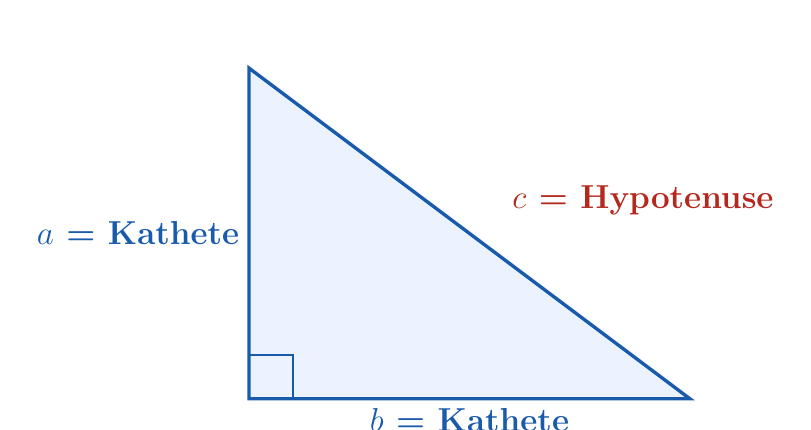
\begin{tikzpicture}[scale=1.4]
  \draw[very thick, mainblue, fill=lightblue!60]
    (0,0) -- (4,0) -- (0,3) -- cycle;
  \draw[mainblue, thick] (0,0) rectangle (0.4,0.4);
  \node[below, font=\large\bfseries, mainblue] at (2,0) {$b$ = Kathete};
  \node[left,  font=\large\bfseries, mainblue] at (0,1.5) {$a$ = Kathete};
  \node[right, font=\large\bfseries, mainred]  at (2.3,1.8) {$c$ = Hypotenuse};
\end{tikzpicture}
\end{center}

\begin{tipbox}
\textbf{Wie erkenne ich die Hypotenuse?} Ganz einfach:\\[0.3cm]
\begin{itemize}
  \item Sie liegt \textbf{gegen\"uber} dem rechten Winkel (dem $\square$)
  \item Sie ist \textbf{immer die l\"angste} Seite
  \item Sie heisst \textbf{immer $c$}
\end{itemize}
\textbf{Eselsbr\"ucke:} Die Hypotenuse ``flieht'' vor dem rechten Winkel -- sie ist so weit wie m\"oglich weg davon!
\end{tipbox}

\newpage

\subsection{Die Formel -- und was sie bedeutet}

\begin{formulabox}
\[
  \boxed{a^2 + b^2 = c^2}
\]
\textbf{In Worten:} Kathete$^2$ + Kathete$^2$ = Hypotenuse$^2$
\end{formulabox}

\begin{visualbox}
\textbf{Warum stimmt das? -- Sieh es einfach so:}\\[0.3cm]
Stell dir vor, du baust auf jede Seite des Dreiecks ein Quadrat.\\
Das Quadrat auf der Hypotenuse ($c^2$) ist \textbf{genauso gross}
wie die beiden anderen Quadrate zusammen ($a^2 + b^2$).

\begin{center}
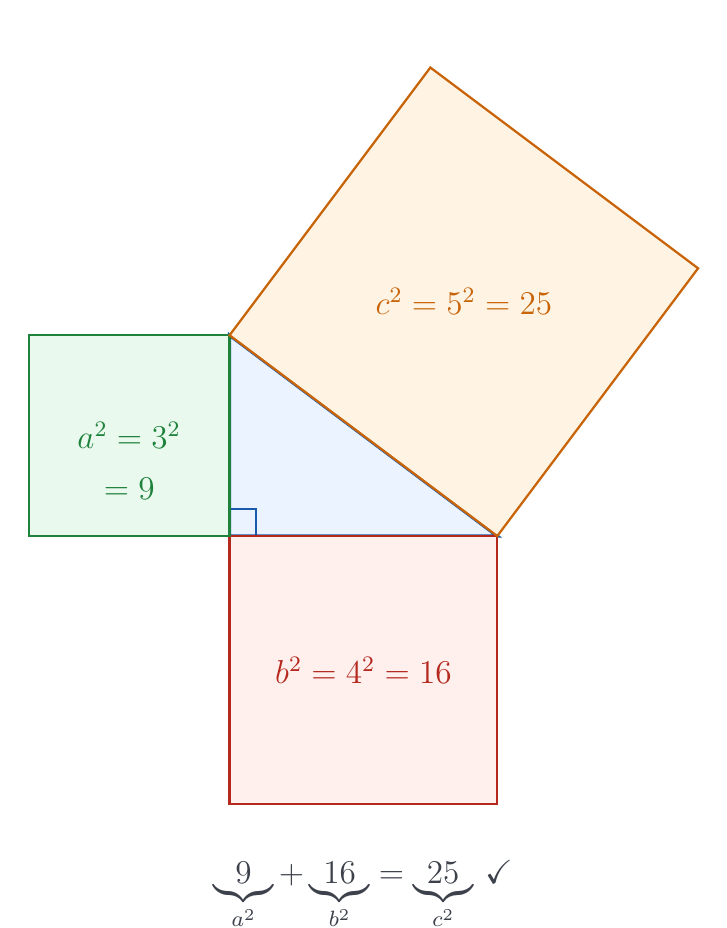
\begin{tikzpicture}[scale=0.85]
  \draw[very thick, mainblue, fill=lightblue!60]
    (3,0) -- (7,0) -- (3,3) -- cycle;
  \draw[mainblue, thick] (3,0) rectangle (3.4,0.4);
  \draw[mainred, thick, fill=lightred!60]
    (3,0) -- (7,0) -- (7,-4) -- (3,-4) -- cycle;
  \node[mainred, font=\bfseries\large] at (5,-2) {$b^2 = 4^2 = 16$};
  \draw[maingreen, thick, fill=lightgreen!60]
    (3,0) -- (3,3) -- (0,3) -- (0,0) -- cycle;
  \node[maingreen, font=\bfseries\large] at (1.5,1.5) {$a^2 = 3^2$};
  \node[maingreen, font=\bfseries\large] at (1.5,0.7) {$= 9$};
  \draw[mainorange, thick, fill=lightorange!70]
    (7,0) -- (3,3) -- (3+3,3+4) -- (7+3,0+4) -- cycle;
  \node[mainorange, font=\bfseries\large] at (6.5,3.5) {$c^2 = 5^2 = 25$};
  \node[below, darkgray, font=\large\bfseries] at (5,-4.7)
    {$\underbrace{9}_{a^2} + \underbrace{16}_{b^2} = \underbrace{25}_{c^2}$ \checkmark};
\end{tikzpicture}
\end{center}
\end{visualbox}

\subsection{Die drei Formeln -- wann benutze ich welche?}

\begin{center}
\renewcommand{\arraystretch}{2.2}
\begin{tabular}{>{\centering\arraybackslash}m{3cm} >{\centering\arraybackslash}m{4cm} >{\centering\arraybackslash}m{5.5cm}}
  \toprule
  \textbf{Was ist gesucht?} & \textbf{Formel} & \textbf{Wann benutzen?} \\
  \midrule
  Hypotenuse $c$ &
  \colorbox{lightred}{$c = \sqrt{a^2 + b^2}$} &
  Ich kenne beide Katheten ($a$ und $b$) \\[0.3cm]
  Kathete $a$ &
  \colorbox{lightgreen}{$a = \sqrt{c^2 - b^2}$} &
  Ich kenne $c$ und $b$ (minus!) \\[0.3cm]
  Kathete $b$ &
  \colorbox{lightgreen}{$b = \sqrt{c^2 - a^2}$} &
  Ich kenne $c$ und $a$ (minus!) \\
  \bottomrule
\end{tabular}
\end{center}

\begin{tipbox}
\textbf{Merke den Unterschied:}\\
$\bullet$ Hypotenuse berechnen $\rightarrow$ \textbf{plus} ($a^2 + b^2$)\\
$\bullet$ Kathete berechnen $\rightarrow$ \textbf{minus} ($c^2 - \ldots$)
\end{tipbox}

\subsection{Schritt-f\"ur-Schritt -- so rechnest du}

\begin{simplebox}
\textbf{Immer in diesen 4 Schritten vorgehen:}

\vspace{0.4cm}
\begin{enumerate}[leftmargin=1.5cm, label=\textbf{Schritt \arabic*:}, itemsep=0.4cm]
  \item \textbf{Zeichne das Dreieck!} Trage alle bekannten Werte ein. Markiere den rechten Winkel.
  \item \textbf{Welche Seite ist gesucht?} Ist es $c$ (Hypotenuse) oder $a$ / $b$ (Kathete)?
  \item \textbf{W\"ahle die richtige Formel} aus der Tabelle oben.
  \item \textbf{Rechne aus und schreibe die Einheit hin!} (cm, m, \ldots)
\end{enumerate}
\end{simplebox}

\subsection{Gerechnete Beispiele}

\begin{examplebox}{Hypotenuse berechnen -- $a = 3$\,cm, $b = 4$\,cm}
\textit{Gesucht: $c$ (die l\"angste Seite)}\\[0.3cm]
Beide Katheten bekannt $\Rightarrow$ \textbf{Plus-Formel}:
\begin{align*}
  c &= \sqrt{a^2 + b^2} = \sqrt{3^2 + 4^2} = \sqrt{9 + 16} = \sqrt{25} = \mathbf{5\,cm}
\end{align*}
\textit{Probe:} $3^2 + 4^2 = 9 + 16 = 25 = 5^2$ \checkmark
\end{examplebox}

\begin{examplebox}{Kathete berechnen -- $c = 10$\,cm, $b = 6$\,cm}
\textit{Gesucht: $a$ (eine Kathete)}\\[0.3cm]
Hypotenuse und eine Kathete bekannt $\Rightarrow$ \textbf{Minus-Formel}:
\begin{align*}
  a &= \sqrt{c^2 - b^2} = \sqrt{10^2 - 6^2} = \sqrt{100 - 36} = \sqrt{64} = \mathbf{8\,cm}
\end{align*}
\textit{Probe:} $8^2 + 6^2 = 64 + 36 = 100 = 10^2$ \checkmark
\end{examplebox}

\begin{examplebox}{Alltagsbeispiel: Leiter an der Wand}
Eine Leiter ist $5$\,m lang. Ihr Fuss steht $3$\,m von der Wand entfernt.
Wie hoch reicht sie?

\begin{center}
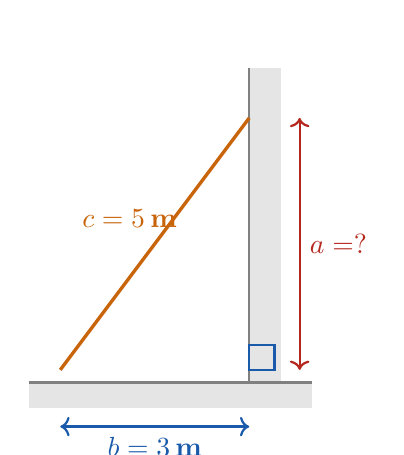
\begin{tikzpicture}[scale=0.8]
  \fill[gray!20] (3,-0.2) rectangle (3.5,4.8);
  \draw[thick, gray] (3,-0.2) -- (3,4.8);
  \fill[gray!20] (-0.5,-0.2) rectangle (4,-0.6);
  \draw[thick, gray] (-0.5,-0.2) -- (4,-0.2);
  \draw[very thick, mainorange] (0,0) -- (3,4);
  \draw[mainblue, thick] (3,0) rectangle (3.4,0.4);
  \draw[<->, mainblue, thick] (0,-0.9) -- (3,-0.9)
    node[midway, below, font=\bfseries] {$b = 3$\,m};
  \draw[<->, mainred, thick] (3.8,0) -- (3.8,4)
    node[midway, right, font=\bfseries] {$a = ?$};
  \node[mainorange, font=\bfseries] at (1.1,2.4) {$c = 5$\,m};
\end{tikzpicture}
\end{center}

\[
  a = \sqrt{c^2 - b^2} = \sqrt{25 - 9} = \sqrt{16} = \mathbf{4\,m}
\]
Die Leiter reicht \textbf{4\,m} hoch.
\end{examplebox}

\begin{examplebox}{Diagonale im Rechteck}
Ein Rechteck ist $6$\,cm breit und $8$\,cm lang. Wie lang ist die Diagonale?

Die Diagonale teilt das Rechteck in zwei rechtwinklige Dreiecke.
Die Diagonale ist die \textbf{Hypotenuse}!
\[
  c = \sqrt{6^2 + 8^2} = \sqrt{36 + 64} = \sqrt{100} = \mathbf{10\,cm}
\]
\end{examplebox}

\begin{fehlerbox}
\begin{itemize}
  \item \textbf{Fehler 1:} Die falsche Seite als Hypotenuse bezeichnen.\\
    $\Rightarrow$ \textit{Hypotenuse ist IMMER gegen\"uber dem rechten Winkel!}
  \item \textbf{Fehler 2:} Kathete berechnen, aber die Plus-Formel benutzen.\\
    $\Rightarrow$ \textit{Kathete berechnen = Minus-Formel!}
  \item \textbf{Fehler 3:} Vergessen, die Wurzel zu ziehen.\\
    $\Rightarrow$ \textit{Am Ende immer $\sqrt{\phantom{x}}$ nicht vergessen!}
  \item \textbf{Fehler 4:} Einheit vergessen.\\
    $\Rightarrow$ \textit{Immer cm, m, km \ldots hinschreiben!}
\end{itemize}
\end{fehlerbox}

\subsection{\"Ubungsaufgaben -- Pythagoras}

\exercise{Ein rechtwinkliges Dreieck hat $a = 6$\,cm und $b = 8$\,cm. Berechne $c$.\\[0.8cm]
  \textit{L\"osung:} \dotfill}

\exercise{$c = 13$\,cm, $a = 5$\,cm. Berechne $b$.\\[0.8cm]
  \textit{L\"osung:} \dotfill}

\exercise{Ein Rechteck ist $9$\,cm breit und $12$\,cm lang. Wie lang ist die Diagonale?\\[0.8cm]
  \textit{L\"osung:} \dotfill}

\exercise{Ein gleichschenkliges Dreieck hat Basis $10$\,cm und Schenkel $13$\,cm.\\
  \textit{Hinweis: Teile das Dreieck in der Mitte!}\\[0.8cm]
  Berechne die H\"ohe: \dotfill}

\exercise{Ein Schiff f\"ahrt $12$\,km nach Norden, dann $5$\,km nach Osten.
  Wie weit ist es nun vom Startpunkt entfernt (Luftlinie)?\\[0.8cm]
  \textit{L\"osung:} \dotfill}

\newpage
% ============================================================
\section{\color{mainblue}Geometrie -- Fl\"achen und K\"orper}
% ============================================================

\subsection{Fl\"acheninhalte}

\begin{formulabox}
\renewcommand{\arraystretch}{1.7}
\begin{tabular}{llll}
  \toprule
  \textbf{Figur} & \textbf{Formel} & & \textbf{Variablen} \\
  \midrule
  Quadrat        & $A = a^2$                       && $a$ = Seitenl\"ange \\
  Rechteck       & $A = l \cdot b$                 && $l$ = L\"ange, $b$ = Breite \\
  Dreieck        & $A = \dfrac{g \cdot h}{2}$      && $g$ = Grundlinie, $h$ = H\"ohe \\
  Parallelogramm & $A = g \cdot h$                 && $g$ = Grundseite, $h$ = H\"ohe \\
  Trapez         & $A = \dfrac{(a+c)\cdot h}{2}$   && $a,c$ = Parallelseiten \\
  Kreis          & $A = \pi \cdot r^2$, $U = 2\pi r$ && $r$ = Radius \\
  \bottomrule
\end{tabular}
\end{formulabox}

\begin{center}
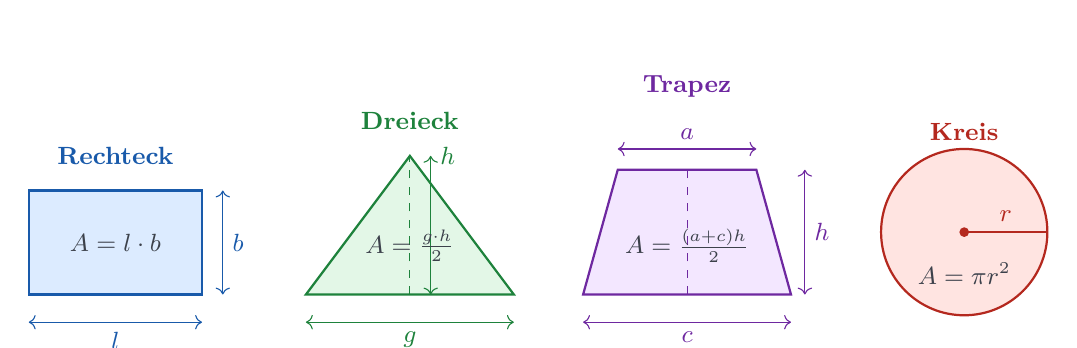
\begin{tikzpicture}[scale=0.88]
  \fill[lightblue] (0,0) rectangle (2.5,1.5);
  \draw[mainblue, thick] (0,0) rectangle (2.5,1.5);
  \draw[<->, mainblue] (0,-0.4) -- (2.5,-0.4) node[midway,below,font=\small]{$l$};
  \draw[<->, mainblue] (2.8,0)  -- (2.8,1.5)  node[midway,right,font=\small]{$b$};
  \node[font=\small\bfseries, mainblue] at (1.25, 2.0) {Rechteck};
  \node[font=\small, darkgray] at (1.25, 0.75) {$A=l \cdot b$};

  \fill[lightgreen!80] (4,0) -- (7,0) -- (5.5,2.0) -- cycle;
  \draw[maingreen, thick] (4,0) -- (7,0) -- (5.5,2.0) -- cycle;
  \draw[dashed, maingreen] (5.5,0) -- (5.5,2.0);
  \draw[<->, maingreen] (4,-0.4) -- (7,-0.4) node[midway,below,font=\small]{$g$};
  \draw[<->, maingreen] (5.8,0) -- (5.8,2.0) node[below,right,font=\small]{$h$};
  \node[font=\small\bfseries, maingreen] at (5.5, 2.5) {Dreieck};
  \node[font=\small, darkgray] at (5.5, 0.7) {$A=\frac{g\cdot h}{2}$};

  \fill[lightpurple!80] (8,0) -- (11,0) -- (10.5,1.8) -- (8.5,1.8) -- cycle;
  \draw[mainpurple, thick] (8,0) -- (11,0) -- (10.5,1.8) -- (8.5,1.8) -- cycle;
  \draw[dashed, mainpurple] (9.5,0) -- (9.5,1.8);
  \draw[<->, mainpurple] (8,-0.4) -- (11,-0.4) node[midway,below,font=\small]{$c$};
  \draw[<->, mainpurple] (8.5,2.1) -- (10.5,2.1) node[midway,above,font=\small]{$a$};
  \draw[<->, mainpurple] (11.2,0) -- (11.2,1.8) node[midway,right,font=\small]{$h$};
  \node[font=\small\bfseries, mainpurple] at (9.5, 3.0) {Trapez};
  \node[font=\small, darkgray] at (9.5, 0.7) {$A=\frac{(a+c)h}{2}$};

  \fill[lightred] (13.5,0.9) circle (1.2cm);
  \draw[mainred, thick] (13.5,0.9) circle (1.2cm);
  \draw[mainred, thick] (13.5,0.9) -- (14.7,0.9)
    node[midway,above,font=\small]{$r$};
  \fill[mainred] (13.5,0.9) circle (0.07cm);
  \node[font=\small\bfseries, mainred] at (13.5, 2.35) {Kreis};
  \node[font=\small, darkgray] at (13.5, 0.3) {$A=\pi r^2$};
\end{tikzpicture}
\end{center}

\subsection{K\"orper -- Volumen und Oberfl\"ache}

\begin{formulabox}
\renewcommand{\arraystretch}{1.8}
\begin{tabular}{lll}
  \toprule
  \textbf{K\"orper} & \textbf{Volumen} & \textbf{Oberfl\"ache} \\
  \midrule
  Quader      & $V = l \cdot b \cdot h$            & $O = 2(lb+lh+bh)$ \\
  W\"urfel     & $V = a^3$                           & $O = 6a^2$ \\
  Zylinder    & $V = \pi r^2 \cdot h$               & $O = 2\pi r^2 + 2\pi r h$ \\
  Kegel       & $V = \frac{1}{3}\pi r^2 \cdot h$    & $O = \pi r^2 + \pi r s$ \\
  Kugel       & $V = \frac{4}{3}\pi r^3$            & $O = 4\pi r^2$ \\
  \textbf{Quadratische Pyramide} & $\mathbf{V = \frac{1}{3} \cdot a^2 \cdot h}$ &
    $\mathbf{O = a^2 + 2 \cdot a \cdot s_M}$ \\
  \bottomrule
\end{tabular}
\end{formulabox}

\subsection{Die Pyramide}

\begin{merkbox}
Eine \textbf{Pyramide} hat eine Grundfl\"ache (meist Quadrat oder Rechteck) und
\textbf{dreieckige Seitenfl\"achen}, die sich in einer \textbf{Spitze} treffen.\\[0.2cm]
Die bekannteste: die \textbf{\"Agyptische Pyramide} -- eine quadratische Pyramide!
\end{merkbox}

\begin{center}
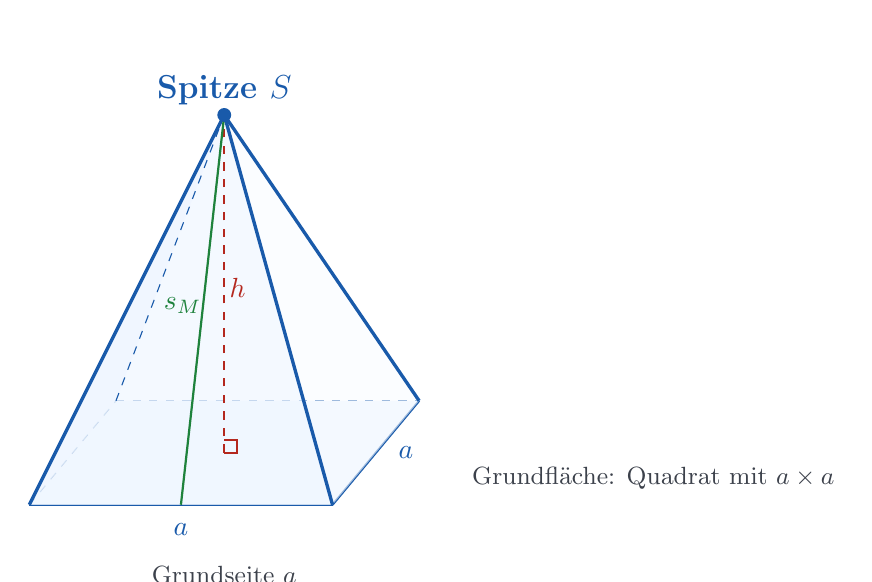
\begin{tikzpicture}[scale=1.1]
  % Base of pyramid (quadrilateral shown in perspective)
  \coordinate (A) at (0,0);
  \coordinate (B) at (3.5,0);
  \coordinate (C) at (4.5,1.2);
  \coordinate (D) at (1.0,1.2);
  % Apex
  \coordinate (S) at (2.25,4.5);

  % Base (dashed back edges)
  \fill[lightblue!60, opacity=0.7] (A) -- (B) -- (C) -- (D) -- cycle;
  \draw[mainblue, thick] (A) -- (B);
  \draw[mainblue, thick] (B) -- (C);
  \draw[mainblue, dashed] (D) -- (C);
  \draw[mainblue, dashed] (A) -- (D);

  % Side faces
  \fill[lightblue!40, opacity=0.8] (A) -- (B) -- (S) -- cycle;
  \fill[lightblue!20, opacity=0.6] (B) -- (C) -- (S) -- cycle;
  \fill[lightblue!50, opacity=0.5] (A) -- (D) -- (S) -- cycle;

  % Visible edges
  \draw[mainblue, very thick] (A) -- (S);
  \draw[mainblue, very thick] (B) -- (S);
  \draw[mainblue, very thick] (C) -- (S);
  \draw[mainblue, dashed]     (D) -- (S);

  % Height
  \coordinate (Mbase) at (2.25,0.6);
  \draw[mainred, thick, dashed] (Mbase) -- (S);
  \draw[mainred, thick] (Mbase) -- ++(0.15,0) -- ++(0,0.15) -- ++(-0.15,0);
  \node[mainred, right, font=\bfseries] at (2.2,2.5) {$h$};

  % Slant height
  \coordinate (Mmid) at (1.75,0);
  \draw[maingreen, thick] (Mmid) -- (S);
  \node[maingreen, left, font=\bfseries] at (2.1,2.3) {$s_M$};

  % Labels
  \node[below, mainblue, font=\bfseries] at (1.75,-0.1) {$a$};
  \node[right, mainblue, font=\bfseries] at (4.15,0.6) {$a$};
  \node[above, mainblue, font=\bfseries\large] at (S) {Spitze $S$};
  \fill[mainblue] (S) circle (0.08);

  % Annotations
  \node[below, darkgray, font=\small] at (2.25,-0.6)
    {Grundseite $a$};
  \node[right, darkgray, font=\small] at (5.0,0.3)
    {Grundfl\"ache: Quadrat mit $a \times a$};
\end{tikzpicture}
\end{center}

\begin{formulabox}
\textbf{Quadratische Pyramide -- Formeln:}
\[
  \boxed{V = \frac{1}{3} \cdot a^2 \cdot h}
  \qquad
  \boxed{O = a^2 + 4 \cdot \frac{a \cdot s_M}{2} = a^2 + 2 \cdot a \cdot s_M}
\]
\begin{itemize}
  \item $a$ = Seitenl\"ange der quadratischen Grundfl\"ache
  \item $h$ = \textbf{H\"ohe} der Pyramide (senkrecht von Spitze zur Mitte der Grundfl\"ache)
  \item $s_M$ = \textbf{Apothema / Schr\"agseite} (senkrechte H\"ohe einer Seitenfl\"ache)
  \item Die \textbf{Schr\"agkante} $s$ verbindet die Spitze mit einer Ecke der Grundfl\"ache
\end{itemize}
\end{formulabox}

\begin{tipbox}
\textbf{Schr\"agseite $s_M$ mit Pythagoras berechnen:}
\[
  s_M = \sqrt{h^2 + \left(\frac{a}{2}\right)^2}
\]
\textbf{Schr\"agkante $s$ mit Pythagoras berechnen:}
\[
  s = \sqrt{h^2 + \left(\frac{a\sqrt{2}}{2}\right)^2} = \sqrt{h^2 + \frac{a^2}{2}}
\]
Das rechtwinklige Dreieck liegt \textbf{innerhalb} der Pyramide!
\end{tipbox}

\begin{examplebox}{Pyramide: $a = 6$\,cm, $h = 4$\,cm}
\textbf{Schr\"agseite berechnen:}
\[
  s_M = \sqrt{4^2 + \left(\frac{6}{2}\right)^2} = \sqrt{16 + 9} = \sqrt{25} = \mathbf{5\,cm}
\]

\textbf{Volumen:}
\[
  V = \frac{1}{3} \cdot 6^2 \cdot 4 = \frac{1}{3} \cdot 36 \cdot 4 = \frac{144}{3} = \mathbf{48\,cm^3}
\]

\textbf{Oberfl\"ache:}
\[
  O = 6^2 + 2 \cdot 6 \cdot 5 = 36 + 60 = \mathbf{96\,cm^2}
\]
\end{examplebox}

\begin{examplebox}{Pyramide von Gizeh -- Realweltbeispiel}
Die grosse Pyramide von Gizeh hat (urspr\"unglich) $a \approx 230$\,m und $h \approx 147$\,m.

\textbf{Volumen:}
\[
  V = \frac{1}{3} \cdot 230^2 \cdot 147 = \frac{1}{3} \cdot 52\,900 \cdot 147 \approx \mathbf{2\,592\,100\,m^3}
\]
Das sind \textbf{rund 2,6 Millionen Kubikmeter} -- ungef\"ahr 1 Million gef\"ullte Badewannen!
\end{examplebox}

\subsection{3D-K\"orper im \"Uberblick}

\begin{visualbox}
\textbf{Alle K\"orper auf einen Blick:}

\begin{center}
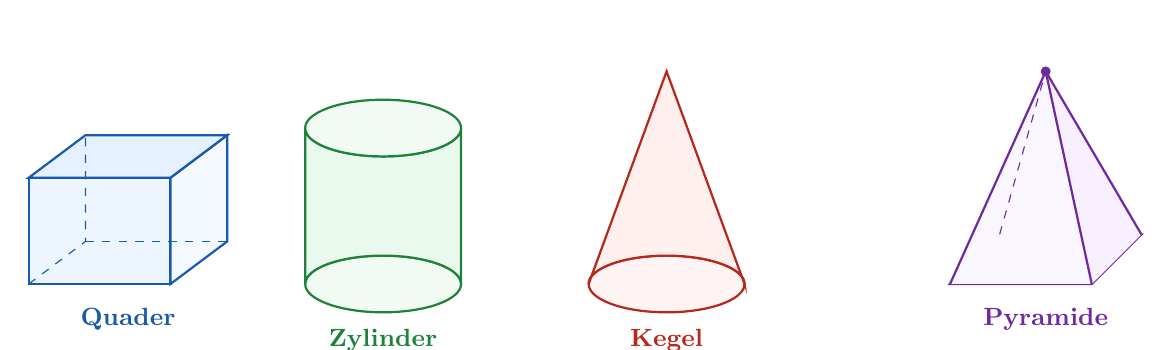
\begin{tikzpicture}[scale=0.9, every node/.style={font=\small}]

  % ─── Quader ───────────────────────────────────────────────
  \begin{scope}[xshift=0cm]
    \draw[mainblue, thick, fill=lightblue!50]
      (0,0,0) -- (2,0,0) -- (2,1.5,0) -- (0,1.5,0) -- cycle;
    \draw[mainblue, thick, fill=lightblue!30]
      (2,0,0) -- (2.8,0.6,0) -- (2.8,2.1,0) -- (2,1.5,0) -- cycle;
    \draw[mainblue, thick, fill=lightblue!70]
      (0,1.5,0) -- (2,1.5,0) -- (2.8,2.1,0) -- (0.8,2.1,0) -- cycle;
    \draw[mainblue, dashed] (0,0,0) -- (0.8,0.6,0) -- (0.8,2.1,0);
    \draw[mainblue, dashed] (0.8,0.6,0) -- (2.8,0.6,0);
    \node[mainblue, font=\small\bfseries] at (1.4,-0.5) {Quader};
  \end{scope}

  % ─── Zylinder ─────────────────────────────────────────────
  \begin{scope}[xshift=5cm]
    \draw[maingreen, thick, fill=lightgreen!40]
      (0,0) ellipse (1.1 and 0.4);
    \draw[maingreen, thick, fill=lightgreen!60]
      (-1.1,0) -- (-1.1,2.2) arc(180:360:1.1 and 0.4) -- (1.1,0)
      arc(0:180:1.1 and 0.4);
    \draw[maingreen, thick, fill=lightgreen!40]
      (0,2.2) ellipse (1.1 and 0.4);
    \node[maingreen, font=\small\bfseries] at (0,-0.8) {Zylinder};
  \end{scope}

  % ─── Kegel ────────────────────────────────────────────────
  \begin{scope}[xshift=9cm]
    \draw[mainred, thick, fill=lightred!40]
      (0,0) ellipse (1.1 and 0.4);
    \draw[mainred, thick, fill=lightred!60]
      (-1.1,0) -- (0,3) -- (1.1,0) arc(0:180:1.1 and 0.4);
    \draw[mainred, dashed] (1.1,0) arc(0:-180:1.1 and 0.4);
    \node[mainred, font=\small\bfseries] at (0,-0.8) {Kegel};
  \end{scope}

  % ─── Pyramide ─────────────────────────────────────────────
  \begin{scope}[xshift=13cm]
    % Base rhombus (perspective)
    \fill[lightpurple!60]
      (0,0) -- (2,0) -- (2.7,0.7) -- (0.7,0.7) -- cycle;
    \draw[mainpurple, thick] (0,0) -- (2,0) -- (2.7,0.7) -- (0.7,0.7) -- cycle;
    % Visible faces
    \fill[lightpurple!30] (0,0) -- (2,0) -- (1.35,3) -- cycle;
    \fill[lightpurple!50] (2,0) -- (2.7,0.7) -- (1.35,3) -- cycle;
    \draw[mainpurple, thick] (0,0) -- (1.35,3);
    \draw[mainpurple, thick] (2,0) -- (1.35,3);
    \draw[mainpurple, thick] (2.7,0.7) -- (1.35,3);
    \draw[mainpurple, dashed] (0.7,0.7) -- (1.35,3);
    \fill[mainpurple] (1.35,3) circle (0.07);
    \node[mainpurple, font=\small\bfseries] at (1.35,-0.5) {Pyramide};
  \end{scope}

\end{tikzpicture}
\end{center}
\end{visualbox}

\begin{examplebox}{Zylinder: $r=5$\,cm, $h=12$\,cm}
\[
  V = \pi \cdot 5^2 \cdot 12 = 300\pi \approx \mathbf{942{,}5\,\text{cm}^3}
\]
\[
  O = 2\pi \cdot 25 + 2\pi \cdot 5 \cdot 12
    = 50\pi + 120\pi = 170\pi \approx \mathbf{534{,}1\,\text{cm}^2}
\]
\end{examplebox}

\subsection{\"Ubungsaufgaben -- Geometrie}

\exercise{Berechne den Fl\"acheninhalt: Dreieck mit $g=10$\,cm und $h=6$\,cm.\\[0.8cm]
  \textit{L\"osung:} \dotfill}

\exercise{Ein Quader: $l=8$\,cm, $b=5$\,cm, $h=3$\,cm. Berechne $V$ und $O$.\\[0.8cm]
  \textit{L\"osung:} \dotfill}

\exercise{Kreis mit $r=7$\,cm: Berechne Fl\"acheninhalt und Umfang.\\[0.8cm]
  \textit{L\"osung:} \dotfill}

\exercise{Ein Trapez hat $a=6$\,cm, $c=10$\,cm und $h=4$\,cm. Berechne den Fl\"acheninhalt.\\[0.8cm]
  \textit{L\"osung:} \dotfill}

\exercise{Eine quadratische Pyramide hat $a = 8$\,cm und $h = 3$\,cm.
  Berechne (a) die Schr\"agseite $s_M$, (b) das Volumen $V$, (c) die Oberfl\"ache $O$.\\[1.5cm]
  \textit{L\"osung:} \dotfill}

\exercise{Ein Kegel hat $r = 4$\,cm und $h = 3$\,cm. Berechne sein Volumen.
  \textit{Hinweis: Die Schr\"agseite $s$ ben\"otigst du f\"ur die Oberfl\"ache: $s = \sqrt{r^2 + h^2}$.}\\[0.8cm]
  \textit{L\"osung:} \dotfill}

\newpage
% ============================================================
\section{\color{mainblue}Prozent- und Zinsrechnung}
% ============================================================

\subsection{Grundformeln}

\begin{formulabox}
\[
  \boxed{W = \frac{p}{100} \cdot G}
  \qquad
  \boxed{p = \frac{W}{G} \cdot 100}
  \qquad
  \boxed{G = \frac{W \cdot 100}{p}}
\]
\begin{itemize}
  \item $W$ = \textbf{Prozentwert} (gesuchter/gegebener Anteil)
  \item $p$ = \textbf{Prozentsatz} (die Prozentzahl in \%)
  \item $G$ = \textbf{Grundwert} (Ausgangsmenge = 100\,\%)
\end{itemize}
\end{formulabox}

\begin{visualbox}
\textbf{Prozentstreifen -- visuelle Hilfe:}

\begin{center}
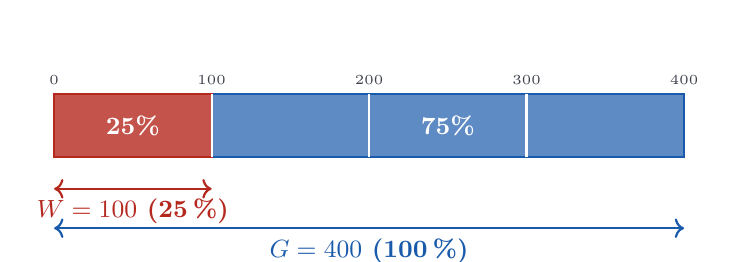
\begin{tikzpicture}[scale=1.0]
  \fill[mainblue!70] (0,0) rectangle (8,0.8);
  \draw[mainblue, thick] (0,0) rectangle (8,0.8);
  \fill[mainred!80] (0,0) rectangle (2,0.8);
  \draw[mainred, thick] (0,0) rectangle (2,0.8);
  \draw[<->, mainred, thick] (0,-0.4) -- (2,-0.4)
    node[midway, below, font=\small\bfseries] {$W=100$ (25\,\%)};
  \draw[<->, mainblue, thick] (0,-0.9) -- (8,-0.9)
    node[midway, below, font=\small\bfseries] {$G=400$ (100\,\%)};
  \node[white, font=\small\bfseries] at (1.0,0.4) {25\%};
  \node[white, font=\small\bfseries] at (5.0,0.4) {75\%};
  \foreach \x in {2,4,6} \draw[white, thick] (\x,0) -- (\x,0.8);
  \node[above, font=\tiny, darkgray] at (0,0.8) {0};
  \node[above, font=\tiny, darkgray] at (2,0.8) {100};
  \node[above, font=\tiny, darkgray] at (4,0.8) {200};
  \node[above, font=\tiny, darkgray] at (6,0.8) {300};
  \node[above, font=\tiny, darkgray] at (8,0.8) {400};
\end{tikzpicture}
\end{center}
\end{visualbox}

\begin{examplebox}{Prozentwert berechnen}
Von 400 Sch\"ulern sind 25\,\% im Sportverein. Wie viele?
\[
  W = \frac{25}{100} \cdot 400 = 0{,}25 \cdot 400 = \mathbf{100}
\]
\end{examplebox}

\begin{examplebox}{Prozentsatz berechnen}
45 von 60 Fragen richtig. Wie viel Prozent?
\[
  p = \frac{45}{60} \cdot 100 = 0{,}75 \cdot 100 = \mathbf{75\,\%}
\]
\end{examplebox}

\begin{examplebox}{Grundwert berechnen}
15\,\% eines Preises sind 60\,\euro. Wie hoch ist der Originalpreis?
\[
  G = \frac{60 \cdot 100}{15} = \mathbf{400\,\text{\euro}}
\]
\end{examplebox}

\subsection{Ver\"anderungen mit Faktor}

\begin{formulabox}
\[
  \text{Erh\"ohung um }p\%:\quad
  \boxed{\text{Neu} = G \cdot \left(1 + \frac{p}{100}\right)}
\]
\[
  \text{Senkung um }p\%:\quad
  \boxed{\text{Neu} = G \cdot \left(1 - \frac{p}{100}\right)}
\]
\end{formulabox}

\begin{examplebox}{Rabatt berechnen}
Ein Fahrrad kostet 350\,\euro, 20\,\% Rabatt:
\[
  350 \cdot (1 - 0{,}20) = 350 \cdot 0{,}8 = \mathbf{280\,\text{\euro}}
\]
\end{examplebox}

\begin{examplebox}{R\"uckw\"artsrechnen -- Originalpreis aus Rabattpreis}
Ein Artikel kostet nach 30\,\% Rabatt noch 140\,\euro. Wie teuer war er vorher?

Der Preis nach Rabatt entspricht 70\,\% des Originalpreises:
\[
  G = \frac{140}{0{,}70} = \mathbf{200\,\text{\euro}}
\]
\textbf{Tipp:} Nicht 30\,\% draufrechnen! Das w\"are $182$ \euro\ -- falsch!
\end{examplebox}

\begin{fehlerbox}
\textbf{H\"aufiger Fehler beim R\"uckw\"artsrechnen:}
Ein Preis wird um 20\,\% gesenkt auf 80\,\euro. Was war der Originalpreis?\\[0.2cm]
\textbf{Falsch:} $80 + 20\,\% = 80 + 16 = 96$ \euro \\
\textbf{Richtig:} $G = \frac{80}{0{,}80} = 100$ \euro
\end{fehlerbox}

\subsection{Zinsrechnung}

\begin{formulabox}
\textbf{Einfache Zinsen:}
\[
  \boxed{Z = \frac{K \cdot p \cdot t}{100}}
\]
\textbf{Zinseszins (nach $n$ Jahren):}
\[
  \boxed{K_n = K \cdot \left(1 + \frac{p}{100}\right)^n}
\]
$K$ = Kapital \quad $p$ = Zinssatz (\%) \quad $t$ = Zeit (Jahre) \quad $n$ = Anzahl Jahre
\end{formulabox}

\begin{examplebox}{Einfache Zinsen}
$K = 5000$\,\euro\ werden zu $p = 2{,}5\,\%$ f\"ur $t = 3$ Jahre angelegt.
\[
  Z = \frac{5000 \cdot 2{,}5 \cdot 3}{100} = \frac{37500}{100} = \mathbf{375\,\text{\euro}}
\]
Endkapital: $5000 + 375 = 5375$\,\euro
\end{examplebox}

\begin{examplebox}{Zinseszins -- Wachstum visualisiert}
$K=2000$\,\euro, $p=3$\,\%, $n=5$ Jahre:
\[
  K_5 = 2000 \cdot 1{,}03^5 \approx \mathbf{2318{,}55\,\text{\euro}}
  \quad\Rightarrow\quad \text{Gewinn: } 318{,}55\,\text{\euro}
\]

\begin{center}
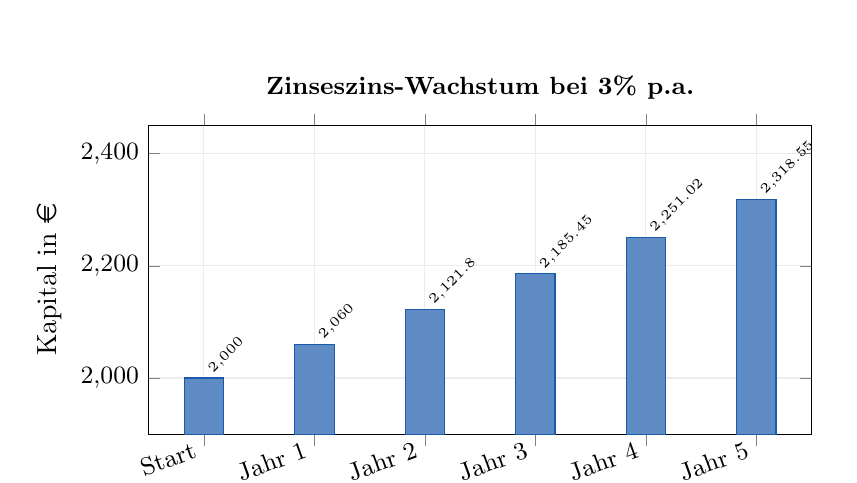
\begin{tikzpicture}
  \begin{axis}[
    width=10cm, height=5.5cm,
    ybar, bar width=0.5cm,
    ymin=1900, ymax=2450,
    xtick={0,1,2,3,4,5},
    xticklabels={Start, Jahr 1, Jahr 2, Jahr 3, Jahr 4, Jahr 5},
    xlabel={}, ylabel={Kapital in \euro},
    nodes near coords,
    nodes near coords style={font=\tiny, rotate=45, anchor=west},
    grid=major, grid style={gray!15},
    title={Zinseszins-Wachstum bei 3\% p.a.},
    title style={font=\small\bfseries},
    x tick label style={font=\small, rotate=20, anchor=east},
    y tick label style={font=\small},
    scaled y ticks=false,
  ]
    \addplot[fill=mainblue!70, draw=mainblue]
      coordinates {
        (0,2000.00)
        (1,2060.00)
        (2,2121.80)
        (3,2185.45)
        (4,2251.02)
        (5,2318.55)
      };
  \end{axis}
\end{tikzpicture}
\end{center}
\end{examplebox}

\newpage

\subsection{\"Ubungsaufgaben -- Prozent \& Zins}

\exercise{Ein Pullover kostet 80\,\euro. Im Sale sind 35\,\% Rabatt. Neuer Preis?\\[0.8cm]
  \textit{L\"osung:} \dotfill}

\exercise{1\,500\,\euro\ werden zu 4\,\% f\"ur 3 Jahre angelegt. Zinsen insgesamt?\\[0.8cm]
  \textit{L\"osung:} \dotfill}

\exercise{Welches Kapital liefert bei 5\,\% in einem Jahr 75\,\euro\ Zinsen?\\[0.8cm]
  \textit{L\"osung:} \dotfill}

\exercise{Ein Preis wird um 10\,\% erh\"oht und dann um 10\,\% gesenkt. Stimmt es, dass
  man wieder beim Ausgangspreis ist? Rechne mit $G = 200$\,\euro\ nach!\\[0.8cm]
  \textit{L\"osung:} \dotfill}

\exercise{Nach einem Rabatt von 25\,\% kostet ein Ger\"at noch 150\,\euro.
  Was war der urspr\"ungliche Preis?\\[0.8cm]
  \textit{L\"osung:} \dotfill}

\exercise{2000\,\euro\ werden f\"ur 4 Jahre zu 3\,\% Zinseszins angelegt.
  Wie viel Geld hat man am Ende?\\[0.8cm]
  \textit{L\"osung:} \dotfill}

\newpage
% ============================================================
\section{\color{mainblue}Daten und Diagramme}
% ============================================================

\subsection{Statistische Kenngr\"ossen}

\begin{formulabox}
\[
  \boxed{\bar{x} = \frac{x_1 + x_2 + \cdots + x_n}{n}}
  \quad\text{(Arithmetisches Mittel / Durchschnitt)}
\]
\begin{itemize}
  \item \textbf{Median:} mittlerer Wert der \textit{sortierten} Reihe;
        bei geradem $n$: Mittelwert der zwei mittleren Werte
  \item \textbf{Modus:} am \textit{h\"aufigsten} vorkommender Wert
  \item \textbf{Spannweite:} $R = x_{\max} - x_{\min}$
\end{itemize}
\end{formulabox}

\begin{tipbox}
\textbf{Schritt-f\"ur-Schritt beim Median:}
\begin{enumerate}
  \item Werte \textbf{aufsteigend sortieren}
  \item Anzahl der Werte z\"ahlen (= $n$)
  \item Wenn $n$ ungerade: mittlerer Wert = Median
  \item Wenn $n$ gerade: Durchschnitt der beiden mittleren Werte = Median
\end{enumerate}
Beispiel (gerades $n$): $2,3,\underbrace{5,7}_{\text{mitte}},9,11$ \quad Median $= \frac{5+7}{2} = 6$
\end{tipbox}

\begin{examplebox}{Alle Kenngr\"ossen berechnen}
Datenreihe: $3,\;7,\;5,\;9,\;5,\;2,\;8$

Sortiert: $2,\;3,\;5,\;\underbrace{\mathbf{5}}_{\text{Median}},\;7,\;8,\;9$
\[
  \bar{x} = \frac{2+3+5+5+7+8+9}{7} = \frac{39}{7} \approx \mathbf{5{,}57}
\]
\[
  \text{Median} = \mathbf{5} \qquad\quad \text{Modus} = \mathbf{5} \qquad\quad R = 9 - 2 = \mathbf{7}
\]

\begin{center}
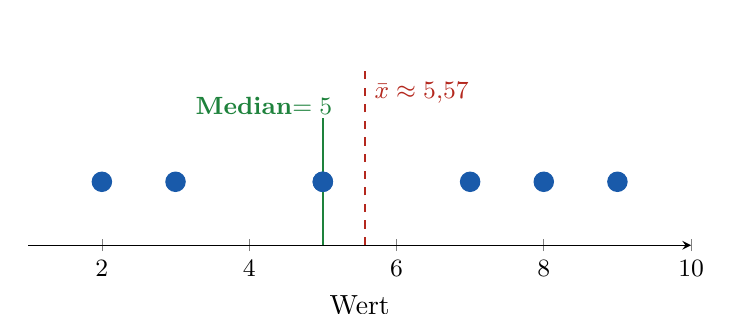
\begin{tikzpicture}
  \begin{axis}[
    width=10cm, height=4cm,
    ymin=0, ymax=1.5,
    xmin=1, xmax=10,
    ytick=\empty,
    xlabel={Wert},
    axis x line=bottom,
    hide y axis,
    tick label style={font=\small},
  ]
    \foreach \v in {2,3,5,5,7,8,9} {
      \addplot[mainblue, mark=*, mark size=3.5pt] coordinates {(\v, 0.5)};
    }
    \addplot[mainred, dashed, thick] coordinates {(5.57,0)(5.57,1.4)};
    \node[mainred, font=\small\bfseries, right] at (axis cs:5.57,1.2)
      {$\bar{x}\approx5{,}57$};
    \addplot[maingreen, thick] coordinates {(5,0)(5,1.0)};
    \node[maingreen, font=\small\bfseries, above] at (axis cs:4.2,0.95)
      {Median$=5$};
  \end{axis}
\end{tikzpicture}
\end{center}
\end{examplebox}

\subsection{H\"aufigkeitstabelle}

\begin{examplebox}{H\"aufigkeitstabelle erstellen}
Noten einer Klasse: $2, 3, 1, 3, 4, 2, 3, 5, 2, 3, 1, 4$

\begin{center}
\renewcommand{\arraystretch}{1.4}
\begin{tabular}{c c c c}
  \toprule
  \textbf{Note} & \textbf{Absolute H\"aufigkeit} & \textbf{Relative H\"aufigkeit} & \textbf{Prozent} \\
  \midrule
  1 & 2 & $\frac{2}{12} \approx 0{,}17$ & 16{,}7\,\% \\
  2 & 3 & $\frac{3}{12} = 0{,}25$       & 25{,}0\,\% \\
  3 & 4 & $\frac{4}{12} \approx 0{,}33$ & 33{,}3\,\% \\
  4 & 2 & $\frac{2}{12} \approx 0{,}17$ & 16{,}7\,\% \\
  5 & 1 & $\frac{1}{12} \approx 0{,}08$ & 8{,}3\,\%  \\
  \midrule
  \textbf{Summe} & \textbf{12} & \textbf{1} & \textbf{100\,\%} \\
  \bottomrule
\end{tabular}
\end{center}
\end{examplebox}

\subsection{Diagrammtypen}

\subsubsection*{S\"aulendiagramm}

\begin{center}
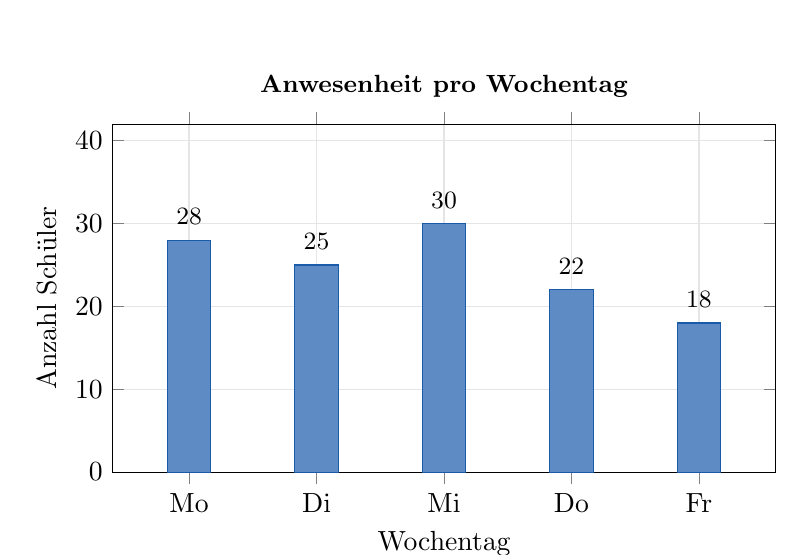
\begin{tikzpicture}
  \begin{axis}[
    width=10cm, height=6cm,
    ybar, bar width=0.55cm,
    ymin=0, ymax=42,
    xtick=data,
    symbolic x coords={Mo,Di,Mi,Do,Fr},
    xlabel={Wochentag}, ylabel={Anzahl Sch\"uler},
    nodes near coords,
    nodes near coords align={vertical},
    nodes near coords style={font=\small\bfseries, yshift=2pt},
    grid=major, grid style={gray!20},
    title={Anwesenheit pro Wochentag},
    title style={font=\small\bfseries},
    enlarge x limits=0.15,
  ]
    \addplot[fill=mainblue!70, draw=mainblue]
      coordinates {(Mo,28)(Di,25)(Mi,30)(Do,22)(Fr,18)};
  \end{axis}
\end{tikzpicture}
\end{center}

\subsubsection*{Liniendiagramm (zeitlicher Verlauf)}

\begin{center}
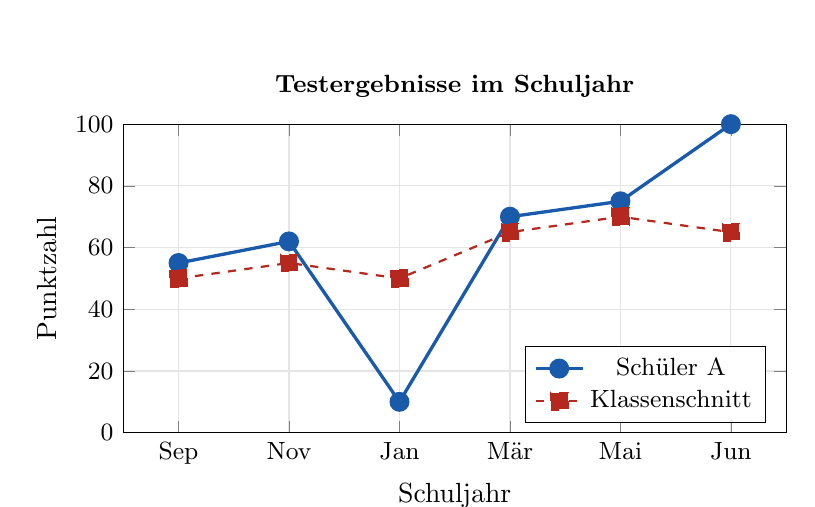
\begin{tikzpicture}
  \begin{axis}[
    width=10cm, height=5.5cm,
    xmin=0.5, xmax=6.5,
    ymin=0, ymax=100,
    xtick={1,2,3,4,5,6},
    xticklabels={Sep, Nov, Jan, M\"ar, Mai, Jun},
    xlabel={Schuljahr}, ylabel={Punktzahl},
    grid=major, grid style={gray!20},
    title={Testergebnisse im Schuljahr},
    title style={font=\small\bfseries},
    mark size=3pt,
    tick label style={font=\small},
    legend pos=south east,
    legend style={font=\small},
  ]
    \addplot[mainblue, very thick, mark=*]
      coordinates {(1,55)(2,62)(3,10)(4,70)(5,75)(6,100)};
    \addplot[mainred, dashed, thick, mark=square*]
      coordinates {(1,50)(2,55)(3,50)(4,65)(5,70)(6,65)};
    \legend{Sch\"uler A, Klassenschnitt};
  \end{axis}
\end{tikzpicture}
\end{center}

\subsubsection*{Kreisdiagramm -- Winkelformel}

\begin{formulabox}
\[
  \boxed{\alpha = \frac{p}{100} \cdot 360^\circ}
\]
Beispiel: $25\% \;\Rightarrow\; \alpha = 0{,}25 \cdot 360^\circ = 90^\circ$
\end{formulabox}

\begin{center}
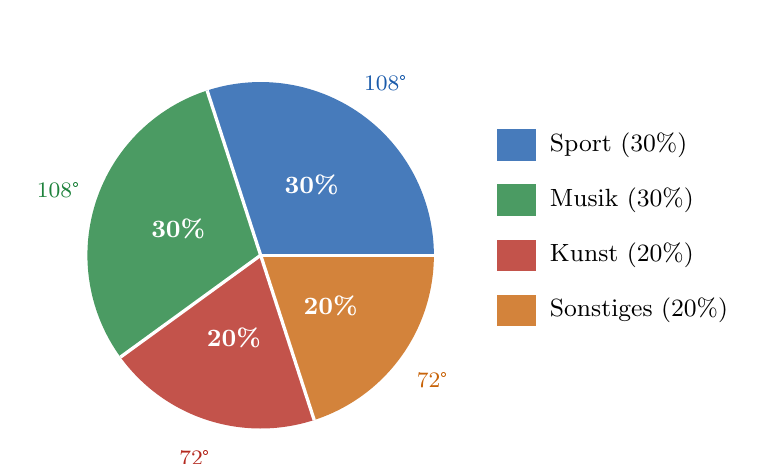
\begin{tikzpicture}[scale=1.0]
  \fill[mainblue!80]   (0,0) -- (2.2,0)
    arc[start angle=0, end angle=108, radius=2.2] -- cycle;
  \fill[maingreen!80]  (0,0) -- ({2.2*cos(108)},{2.2*sin(108)})
    arc[start angle=108, end angle=216, radius=2.2] -- cycle;
  \fill[mainred!80]    (0,0) -- ({2.2*cos(216)},{2.2*sin(216)})
    arc[start angle=216, end angle=288, radius=2.2] -- cycle;
  \fill[mainorange!80] (0,0) -- ({2.2*cos(288)},{2.2*sin(288)})
    arc[start angle=288, end angle=360, radius=2.2] -- cycle;
  \foreach \a in {0,108,216,288}
    \draw[white, very thick] (0,0) -- ({2.2*cos(\a)},{2.2*sin(\a)});
  \node[white, font=\small\bfseries] at ({1.1*cos(54)},{1.1*sin(54)})   {30\%};
  \node[white, font=\small\bfseries] at ({1.1*cos(162)},{1.1*sin(162)}) {30\%};
  \node[white, font=\small\bfseries] at ({1.1*cos(252)},{1.1*sin(252)}) {20\%};
  \node[white, font=\small\bfseries] at ({1.1*cos(324)},{1.1*sin(324)}) {20\%};
  \node[mainblue, font=\footnotesize] at ({2.7*cos(54)},{2.7*sin(54)})   {108°};
  \node[maingreen, font=\footnotesize] at ({2.7*cos(162)},{2.7*sin(162)}) {108°};
  \node[mainred, font=\footnotesize] at ({2.7*cos(252)},{2.7*sin(252)}) {72°};
  \node[mainorange, font=\footnotesize] at ({2.7*cos(324)},{2.7*sin(324)}) {72°};
  \fill[mainblue!80]   (3.0, 1.2) rectangle (3.5, 1.6);
  \node[right, font=\small] at (3.55, 1.4) {Sport (30\%)};
  \fill[maingreen!80]  (3.0, 0.5) rectangle (3.5, 0.9);
  \node[right, font=\small] at (3.55, 0.7) {Musik (30\%)};
  \fill[mainred!80]    (3.0,-0.2) rectangle (3.5, 0.2);
  \node[right, font=\small] at (3.55, 0.0) {Kunst (20\%)};
  \fill[mainorange!80] (3.0,-0.9) rectangle (3.5,-0.5);
  \node[right, font=\small] at (3.55,-0.7) {Sonstiges (20\%)};
\end{tikzpicture}
\end{center}

\subsubsection*{Boxplot -- Einf\"uhrung}

Ein \textbf{Boxplot} zeigt auf einen Blick, wie Daten verteilt sind.

\begin{visualbox}
\begin{center}
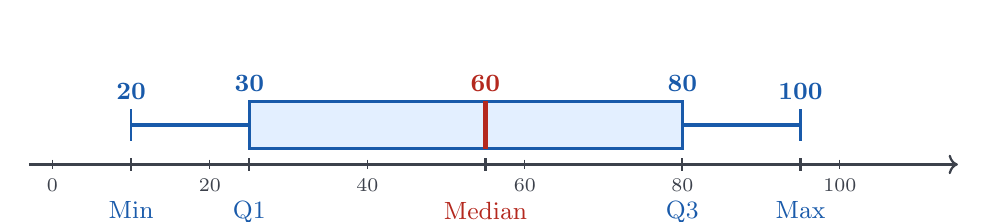
\begin{tikzpicture}
  % Draw on a clean coordinate system, well-spaced
  % Axis line
  \draw[->, thick, darkgray] (-0.3,0) -- (11.5,0);

  % Tick marks and VALUE labels (on axis)
  \foreach \xpos/\val in {1/20, 2.5/30, 5.5/60, 8/80, 9.5/100} {
    \draw[darkgray, thick] (\xpos, 0.08) -- (\xpos, -0.08);
  }
  % Axis scale ticks (0,20,40,...,100)
  \foreach \xpos/\lab in {0/0, 2/20, 4/40, 6/60, 8/80, 10/100} {
    \draw[darkgray] (\xpos, 0.06) -- (\xpos, -0.06)
      node[below, font=\scriptsize, darkgray] {\lab};
  }

  % Whiskers (horizontal lines at mid-height)
  \draw[mainblue, very thick] (1.0, 0.5) -- (2.5, 0.5);   % left whisker
  \draw[mainblue, very thick] (8.0, 0.5) -- (9.5, 0.5);   % right whisker
  % End caps
  \draw[mainblue, thick] (1.0, 0.3) -- (1.0, 0.7);
  \draw[mainblue, thick] (9.5, 0.3) -- (9.5, 0.7);

  % Box (Q1=2.5 to Q3=8.0)
  \fill[lightblue!80] (2.5, 0.2) rectangle (8.0, 0.8);
  \draw[mainblue, very thick] (2.5, 0.2) rectangle (8.0, 0.8);

  % Median line
  \draw[mainred, very thick, line width=2pt] (5.5, 0.2) -- (5.5, 0.8);

  % VALUE labels above
  \node[above, mainblue, font=\small\bfseries] at (1.0, 0.7) {20};
  \node[above, mainblue, font=\small\bfseries] at (2.5, 0.8) {30};
  \node[above, mainred,  font=\small\bfseries] at (5.5, 0.8) {60};
  \node[above, mainblue, font=\small\bfseries] at (8.0, 0.8) {80};
  \node[above, mainblue, font=\small\bfseries] at (9.5, 0.7) {100};

  % NAMED labels below (well below to avoid overlap)
  \node[below=10pt, mainblue, font=\small] at (1.0, 0) {Min};
  \node[below=10pt, mainblue, font=\small] at (2.5, 0) {Q1};
  \node[below=10pt, mainred,  font=\small] at (5.5, 0) {Median};
  \node[below=10pt, mainblue, font=\small] at (8.0, 0) {Q3};
  \node[below=10pt, mainblue, font=\small] at (9.5, 0) {Max};
\end{tikzpicture}
\end{center}
\vspace{0.3cm}
\textbf{Minimum} = kleinster Wert \quad \textbf{Q1} = unteres Viertel \quad \textbf{Median} = Mitte\\
\textbf{Q3} = oberes Viertel \quad \textbf{Maximum} = gr\"osster Wert
\end{visualbox}

\newpage

\subsection{\"Ubungsaufgaben -- Daten \& Diagramme}

\exercise{Notenliste: $2,\;4,\;3,\;1,\;5,\;3,\;2,\;3,\;4,\;2$.
  Berechne Mittelwert, Median, Modus und Spannweite.\\[0.8cm]
  \textit{L\"osung:} \dotfill}

\exercise{In einer Klasse w\"ahlen 40\,\% Sport, 25\,\% Musik, 20\,\% Kunst und 15\,\% Sonstiges.
  Berechne alle Winkel f\"ur ein Kreisdiagramm.\\[1.5cm]}

\exercise{Die Temperaturen einer Woche betragen:
  $12^\circ, 15^\circ, 11^\circ, 9^\circ, 14^\circ, 18^\circ, 20^\circ$.
  Berechne Mittelwert und Median. Was ist die Spannweite?\\[0.8cm]
  \textit{L\"osung:} \dotfill}

\exercise{Erstelle eine H\"aufigkeitstabelle f\"ur die Werte: $1, 2, 2, 3, 1, 4, 2, 3, 5, 1, 2, 4$.
  Welcher Wert ist der Modus?\\[3.0cm]}

\newpage
% ============================================================
\section{\color{mainblue}Formelsammlung -- Alle Themen}
% ============================================================

\begin{center}
\renewcommand{\arraystretch}{1.8}
\begin{tabular}{>{\bfseries\color{mainblue}}p{3.8cm} p{9.5cm}}
  \toprule
  Thema & Wichtigste Formeln \\
  \midrule
  Gleichungen     &
    $ax+b=c \;\Rightarrow\; x=\dfrac{c-b}{a}$ \quad Klammerterm: $a(b+c)=ab+ac$ \\
  Lineare Fkt.    &
    $y=mx+b$ \quad $m=\dfrac{y_2-y_1}{x_2-x_1}$ \quad Nullstelle: $y=0$ setzen \\
  Quadr. Fkt.     &
    $y = ax^2 + bx + c$ \quad $a>0$: Parabel nach oben, $a<0$: nach unten \\
  Winkel          &
    Nebenwinkel: $\alpha+\beta=180^\circ$ \quad Scheitelwinkel: gleich gross \\
                  &
    Stufenwinkel (F): gleich \quad Wechselwinkel (Z): gleich \\
                  &
    Dreieck: $\alpha+\beta+\gamma = 180^\circ$ \\
  Pythagoras      &
    $a^2+b^2=c^2$ \quad
    $c=\sqrt{a^2+b^2}$ \quad
    $a=\sqrt{c^2-b^2}$ \\
  Fl\"achen        &
    Dreieck: $\dfrac{g\cdot h}{2}$ \quad
    Kreis: $\pi r^2$ \quad
    Trapez: $\dfrac{(a+c)h}{2}$ \\
  Volumen         &
    Quader: $l\cdot b\cdot h$ \quad
    Zylinder: $\pi r^2 h$ \quad
    Pyramide: $\dfrac{1}{3}a^2 h$ \\
  Prozent         &
    $W=\dfrac{p}{100}\cdot G$ \quad
    $p=\dfrac{W}{G}\cdot 100$ \quad
    $G=\dfrac{W\cdot 100}{p}$ \\
  Zinsrechnung    &
    $Z=\dfrac{K\cdot p\cdot t}{100}$ \quad
    Zinseszins: $K_n=K\cdot\left(1+\dfrac{p}{100}\right)^n$ \\
  Statistik       &
    $\bar{x}=\dfrac{\sum x_i}{n}$ \quad
    Kreisdiagramm: $\alpha=\dfrac{p}{100}\cdot360^\circ$ \\
  \bottomrule
\end{tabular}
\end{center}

\vspace{0.6cm}
\begin{tipbox}
\begin{itemize}
  \item Immer die \textbf{Probe} machen bei Gleichungen! ($x$ einsetzen und pr\"ufen)
  \item \textbf{Einheiten} nie vergessen: cm, cm$^2$, cm$^3$, \%, \euro
  \item Die Hypotenuse ist \textbf{immer} die l\"angste Seite -- gegen\"uber dem rechten Winkel!
  \item Taschenrechner: die $\pi$-Taste benutzen (nicht $3{,}14$).
  \item Zwischenrechnungen \textbf{aufschreiben} -- es gibt Teilpunkte!
  \item Beim Ablesen von Graphen: Einheiten auf den Achsen beachten!
  \item Steigungsdreieck: zuerst den \textbf{Schritt rechts} ablesen, dann den \textbf{Schritt hoch}.
  \item Winkel an Parallelen: F = Stufen (gleich), Z = Wechsel (gleich)!
  \item Pyramide: das $\frac{1}{3}$ im Volumen \textbf{nicht} vergessen!
\end{itemize}
\end{tipbox}
\vspace{0.4cm}

\begin{merkbox}
\textbf{Schnellcheck vor der Abgabe:}
\begin{enumerate}
  \item Habe ich die Aufgabe vollst\"andig beantwortet?
  \item Sind alle Einheiten dabei?
  \item Ist das Ergebnis sinnvoll (z.B. keine negative L\"ange, kein Winkel $> 360^\circ$)?
  \item Habe ich die Probe gemacht?
  \item Habe ich den richtigen Winkeltyp benannt (Stufen/Wechsel/Scheitel/Neben)?
\end{enumerate}
\end{merkbox}

\end{document}

% Dear Kinds, Please be greatefull for this peace of horror that I made... Yes it's made with AI (Some of it at least), some parts by me, BUT PLEASE THIS THING KILLED ME SO USE IT GREATFULLY Thank you
% also I needed to work in lightmode because there was no darkmode... :) AAAAAAAAAAAAAAAAAA
% - Gavrilo
